
\documentclass[12pt, a4paper]{article}
\usepackage{ragged2e}
\usepackage[margin=1in]{geometry}
\usepackage[utf8]{inputenc}
\usepackage[capposition=top]{floatrow}
%\usepackage[tablesfirst,nolists]{endfloat}
\usepackage{times}
\usepackage[flushleft]{threeparttable}
\usepackage{hyperref}
\usepackage{authblk}
\usepackage{setspace}
\usepackage{apacite}
\usepackage{url}
\usepackage{caption}
\usepackage{graphicx}
\usepackage{titlesec}
\usepackage{color}
\usepackage{endnotes}
\usepackage{caption}
\usepackage{textcase}
\usepackage{booktabs}
\usepackage{titling}
\usepackage{rotating}
\usepackage{amsmath}
\usepackage{bm}
\usepackage{authblk}
\usepackage{adjustbox}
\usepackage[section]{placeins}
\usepackage[toc,page]{appendix}
\usepackage{parskip}

\newcommand{\AT}[1]{\textcolor{red}{AT: #1}}
\newcommand{\NS}[1]{\textcolor{green}{NS: #1}}
\newcommand{\TM}[1]{\textcolor{springgreen3}{TM: #1}}



\captionsetup{
  labelsep=newline,
  justification=raggedright,
  singlelinecheck=false
}

\pagestyle{myheadings}
\title{}
\author{}
\date{}
\doublespacing
%\renewcommand{\efloatheading}[1]{}


\titleformat{name=\section,numberless}[hang]
   {\bfseries}{}{6pt}{\Large}


\let\footnote=\endnote
\newcommand{\vect}[1]{\boldsymbol{#1}}

\bibliographystyle{apacite}
\begin{document}

\title{The link between national football tournaments and domestic abuse - evidence from England}

\author{Anna Trendl$^{a,*}$ \\ \href{mailto:a.trendl@warwick.ac.uk}{a.trendl@warwick.ac.uk}\\
 \and Neil Stewart$^b$ \\ 
 \href{mailto:neil.stewart@wbs.ac.uk}{Neil.Stewart@wbs.ac.uk}
 \\ 
 \and Timothy L. Mullett$^b$ \\
 \href{mailto:Tim.Mullett@wbs.ac.uk}{Tim.Mullett@wbs.ac.uk}
 \\}
 
\date{
    $^a$Department of Psychology, University of Warwick, University Road, Coventry, CV4 7AL, United Kingdom\\
    $^b$Warwick Business School, University of Warwick, Scarman Road, Coventry, CV4 7AL, UK\\
    $^*$Corresponding author\\[2ex]%
    \today
}



\begin{titlepage}
%The cover page should include the title, running head, all authors’ names and affiliations (including departments), and full contact information for the corresponding author.

\maketitle
\thispagestyle{empty}
\centering
This research was funded in part by Economic and Social Research Council grants ES/K002201/1, ES/P008976/1, and ES/N018192/1, and Leverhulme Trust grant RP2012-V-022. 
\clearpage
\thispagestyle{empty}
\RaggedRight
%\begin{center}
%\LARGE{The link between national football tournaments and alcohol-related domestic abuse - evidence from England}
%\end{center}
%\begin{abstract}
%\noindent

%The abstract should be on a separate page and be no longer than 150 words. Five to seven relevant keywords should be listed directly under the abstract on the same page.


%\textbf{Background.} Domestic abuse is increasingly recognised as a serious public health concern worldwide. In the context of England, previous research has suggested that the number of domestic abuse cases reported to the police increase on days when the national football (soccer) team participates in international football tournaments such as the World Cup. Alcohol is hypothesized to be an important factor in this relationship, but its exact role has not been explored yet. We sought to fill this gap by investigating the extent to which alcohol contributes to the link between football and domestic abuse.


%\textbf{Methods.} Using a detailed crime dataset recorded between 2010 and 2018 by the second largest police force in England, we conducted a series of negative binomial regressions to investigate the relationship between England's participation in national football tournaments and the daily number of recorded alcohol-related domestic abuse incidents.


%\textbf{Findings.} Our results show that the number of reported alcohol-related domestic abuse cases increases by 61\%, 95\% CI [32\% -- 96\%] following an England victory, while there is no comparable increase in the number of non-alcohol related domestic abuse cases. This is a large effect, translating into a 0.43 increase in the daily rate of alcohol-related cases per 100,000 individuals, against a base rate 0.71 cases per 100,000. This effect is specific to male-to-female cases, \TM{Delete if analysis not included} survives various robustness checks, and its time course is strongly consistent with a causal link between England's victory and an increase in alcohol-related domestic abuse.


%\textbf{Interpretation.} Alcohol plays an instrumental role in the link between football and domestic abuse. Temporally targeted campaigns could be effective in raising awareness of the adverse effect of football-induced alcohol consumption on the prevalence of domestic abuse.


%\textbf{Funding.} None.
%\end{abstract}

%\newpage
%\thispagestyle{empty}
%\textit{\textbf{Research in context}}


%\textbf{Evidence before this study} While the link between football, masculinity and domestic abuse have been the focus of considerable scientific research, the exact role of alcohol in this relationship has not been explored yet. We searched the Wiley Online Library, Web of Science, and Google Scholar databases using the search terms \textit{football} and \textit{domestic abuse}, covering the period between 1995 and 2019. We have identified two relevant quantitative studies investigating the link between international football tournaments and domestic abuse, both of which used data from England. One study, using data from the 2010 World Cup, has found that the number of recorded domestic abuse cases increased significantly on England win and loss days, compared to various baseline days. Another study used data from the period of the 2002, 2006, and 2010 World Cups, and found that the number of recorded intimate partner violence cases increase 38\% when England loses, and 26\% when England wins or draws, compared to non-match days. To the best of our knowledge, our study is the first to explore the specific role of alcohol in the nexus between football and domestic abuse.


%\textbf{Added value of this study}
%Using 8 years' worth of detailed crime data from the third largest police force in England, we conducted the most comprehensive investigation of the link between football, alcohol, and domestic abuse up to date, and show that England's participation in international football tournaments results in an increase in the number of alcohol-related domestic abuse cases recorded by the police. We show that the time course of this increase is highly consistent with a causal link between football and alcohol-related domestic abuse. Furthermore, we reconcile our findings with previous, seemingly conflicting results, and demonstrate that it is an England victory, and not and England loss that results in an increase in the number of alcohol-related domestic abuse cases. Our results contribute to the scientific understanding of the factors precipitating domestic abuse.

%\textbf{Implications of all the available evidence}
%Alcohol consumption is key to the link between football and domestic abuse in England. Public information campaigns raising awareness of this problem could be the first step to reduce the public health risk associated with increased alcohol consumption following an England victory.

\end{titlepage}



\newpage
\RaggedRight
\section{Introduction}


Domestic abuse is increasingly recognised as a major public policy concern in many countries, including the UK \cite{ep}. While anyone can become a victim of domestic abuse, women are disproportionately affected, with more than 25\% of women, and 15\% of men in England and Wales reported to have experienced some form of domestic abuse since the age of 16 \cite{ONS}.

The link between sporting events and domestic abuse has been the focus of a number of smaller studies \cite{Williams2014}, but large-scale quantitative investigations of this relationship are relatively scarce. In England, previous studies have focused on the link between football (soccer) and domestic abuse. Football's history is inextricably linked to England, and it is by far the most popular sport in the country \cite{Parry2014}, with the 2018 World Cup attracting a record number of 44.5 million viewers \cite{BBC}. These studies have found significant increases in the number of domestic abuse cases recorded by the police on England win, and particularly on England loss days \cite{Brimicombe2012, Kirby2014}. While domestic abuse is predominantly understood as a pattern of ongoing behaviour involving a series of occurrences, rather than a one-off incident triggered by football \cite{Brooks-Hay2018}, these studies, and other qualitative investigations \cite{Swallow} nevertheless suggest that national football tournaments can create an environment where domestic abuse is more likely to occur.


%Two studies have investigated the effect of England's participation in the World Cup on the number of reported domestic abuse incidents. Using data on the number of reported domestic abuse cases in the month of the 2010 World Cup tournament, one study has found that the number of reported domestic abuse cases increased significantly when England lost or won (about 33-35\%), but did not change on days when they drew \cite{Brimicombe2012}. Another study has used daily count data from the 2002, 2006 and 2010 World Cups, and found a 38\% increase in the number of reported domestic violence cases when the England team lost, and a 26\% increase when they won or drew \cite{Kirby2014}. These figures were also quoted in a poster campaign launched before the 2018 World Cup, aiming to raise awareness of the link between football and domestic abuse \cite{NCDV}. While domestic abuse is predominantly understood as a pattern of ongoing behaviour involving a series of occurrences, rather than a one-off incident triggered by football \cite{Brooks-Hay2018}, these studies, and other qualitative investigations \cite{Swallow} nevertheless suggest that national football tournaments can create an environment for abusers that is conducive to domestic abuse.


Why would national football tournaments, such as the World Cup or the European Championship precipitate domestic abuse? England's participation in these tournaments are times of heightened patriotic emotions and a strengthened sense of ``Englishness'', fuelled by media narratives that often use war references, and an ``us vs. them'' rhetoric to generate and represent an English national identity \cite{Vincent2014}. Previous qualitative research has suggested that televised contact sports can serve as vehicle for the male sports fan to redefine, and express his masculinity in a way that allows dominance, control, and can ultimately manifest in the perpetration of domestic abuse \cite{Sabo,Swallow}, given susceptibility to such behaviours. We speculate that this observation is especially pertinent in the context of England's participation in national football tournaments, owing to the popularity of the sport in the country, the associated media attention, and the resulting heightened sense of national consciousness. \AT{Not sure if it would be worth adding something on the link between nationalism and masculinity? It would be good to offer a story for potential pathways whilst avoiding having to say something strong which can be attacked} \TM{I lean towards no}


Previous studies found a strong link between alcohol and domestic abuse, suggesting that alcohol can either be seen as a contributing cause, an aggravating factor, or a trigger of violent behaviour in domestic (and other) settings \cite{Leonard2017}. The ecological model of intimate partner violence (IPV; the most common form of domestic abuse) sees IPV as a product of societal, community, relationship, and individual influences. From a community perspective, \citeA{Graham2017} argue that social contexts where excessive drinking is encouraged (e.g., through the promotion of alcohol during sporting events) are often permissive of violent behaviour and sexism, which can increase the likelihood of alcohol-related domestic abuse. However, strong inhibitory factors (e.g., social norms, and more specifically the condemnation of peers) can offset the disinhibitory effect of alcohol consumption, and reduce the likelihood of subsequent perpetration.  

%Qualitative investigations suggest that alcohol has a strong association with domestic abuse \cite{Peralta2010}: those with alcohol-problems are more likely to be perpetrators and, when alcohol is involved, there is evidence that the violence might result in more serious injuries. However, it is generally understood that the role of alcohol should be considered in the context of a range of social, biological and pyschological factors, and that alcohol is not the direct cause of domestic abuse \cite{Javaid2015,Peralta2010}. 


%It has been suggested that for some men, drinking and violence plays an instrumental role in the construction and expression of masculinity, especially when the problem of masculine deficiency is present (e.g., by unemployment; \cite{Peralta2010}), some perpetrators use alcohol as a ``shield'' that protects them from being seen as a violent abuser and deflect responsibility \cite{Javaid2015}. 


Despite the evident links between alcohol and domestic abuse, the role alcohol plays in the link between football and domestic abuse has not yet been explored in a large-scale quantitative study. Given the strong association between drinking culture and football in England \cite{Dixon2014}, a relationship continuously reinforced by the marketing practices of the alcohol industry \cite{Gornall2014}, we conjecture that alcohol acts as an aggravating factor in the link between football and domestic abuse in England. Exploring the role alcohol plays in this relationship will deepen our understanding of the pathway through which football increases propensity for violence in domestic settings.

To test this hypothesis, we investigate whether the daily number of reported alcohol and non-alcohol related domestic abuse cases recorded by the third largest police force in England (West Midlands Police; WMP) between 2010 and 2019 increase on days when the England national team plays in a national football tournament (the FIFA World Cup and UEFA European Football Championship), and whether the effect, if any, depends on the result of the match.

\citeA{Card2011} had to rely upon the stochastic nature of game outcomes (after controlling for bookmakers expectations) to make a causal inference between unexpected losses in college football and domestic abuse. 
Here, we exploit the fact that national teams are randomly allocated to slots in the tournament structure.
These slots are assigned to dates \emph{before} the teams are are allocated.
Allocation of teams is by the random draw of balls from an urn---the canonical definition of random. 
Thus we can make causal claims about the effect of England matches on domestic abuse.
Our dataset covers a decade, allowing us to conduct a thorough investigation of the characteristics and temporal pattern of the domestic abuse perpetrated on England match days, and extend our findings to understand various characteristics of this relationship. 
We also test the robustness of the effect using various model specifications, time periods, and geographical areas. 



\section{West Midlands Crime Dataset}


Our dataset comprises all incidents and crimes recorded by the West Midlands Police (WMP) in the period between January 1, 2010 and October 10, 2019 (3570 days). The WMP is the second largest police force in England \cite{Homeoffice}, serving an area with a population over 2.9 million in 2018 \cite{populationfigure}. 

The WMP records all reported cases in two databases: incidents and crimes. The incidents database records all reports from officers and the public to call centres and police stations. The crimes database includes all cases which, after initial investigation are found to meet the defenition of a notifiable offence \citeNP{HomeOffice2019}, or fall into one of the special categories of "non-crime". These special categories include rape, domestic abuse, child abuse, racially or religiously aggravated cases, and are recorded (e.g. as ``domestic violence incident - non crime'') in the crimes database, even if the investigation finds that they do not qualify as a notifiable offence (e.g. due to lack of evidence).
 
We focus our analyses on the crimes database, as these have been investigated by police. These records therefore contain more data and are more robust and reliable than incident logs. Officers record the age, gender and ethnicity for both victim and offender (note that the victim offender roles are judged and defined by the recording officer), as well as the location and exact time of the crime. 
In identifying which crimes constitute domestic abuse we include all crime records for specific domestic abuse crimes and non-crimes. There are also a number of crimes which are recorded as non-domestic abuse offences, but which are, or result from domestic abuse. For example, offences of grievous bodily harm. To ensure we identify such cases, we link the records in the crimes database to that of the incidents data. The incidents database contains flags for a number of properties of the incidents \citeNP{HomeOffice2011}, one of which is domestic abuse. Thus, any non-domestic abuse crimes were identified as domestic abuse if they also had such a domestic abuse flag in a linked incident record.

When identifying whether alcohol was involved, we primarily rely upon the specific alcohol flag in the crime record. When an officer records a crime, they must select any flags that are relevant to the case and one of these is "Alcohol Involvement". THe defenition for this is prescribed by the UK home office ``any notifiable offence (crime) where it is perceived, by the victim or any other person, that the effects of alcohol consumption on the offender or victim was an aggravating factor'' \cite{Office2019}. Note that this definition applies to the incident in general, not to either the offender or victim specifically. Since this flag must be actively selected by the recording officer, there is a potential for under reporting. To ameliorate this, we also examined the free text records of the associated incident log. If any linked incident record contained the keyword "alcohol*" \TM{Which sepcific set of keywords did we use?} then it was also identified as alcohol related.
 
 
 
 \TM{ I think get rid of all of this:
 
Most reported cases will be initially recorded as an incident (and then later might be also recorded as a crime after investigation), with a smaller fraction immediately recorded as crime (if it is clear that it meets the criteria for notifiable offences, \citeNP{HomeOffice2019} \citeNP{HomeOffice2019}). For this reason, some recorded crimes will have matching incident entries, while others will not. As an exception, specific types of reported cases (e.g., rape, domestic abuse, child abuse, racially or religiously aggravated cases) that do not qualify as a crime after being investigated (e.g., due to lack of evidence), still get recorded in the crimes database with the indicator ``non crime'' (e.g., ``domestic violence incident - non crime'').


The incidents dataset contains a list of markers capturing various key aspects of the reported case, which are recorded in the call centre when the case is being reported. Most of these markers are common across police forces in England (e.g., domestic abuse, alcohol, drugs, mental health, etc.; \citeNP{HomeOffice2011}). 
These then could be used to assess the severity of case (and support the decision as to whether police attendance is required). 
In contrast, each case in the crimes dataset had been attended by the police, and therefore contains detailed information about the offence that took place, the gender, age, and ethnicity of the victim and offender, and the location and exact time of the crime. 
The role of the victim and the offender was determined by the police. 
A separate alcohol marker exists in the crimes dataset.

Given that much more information is recorded about crimes than incidents, we decided to restrict our analysis to entries in the crimes dataset (i.e., cases that have been investigated by the police), and use only matching entries from the incidents dataset (if any), which provide additional useful call centre-recorded information about the nature of each case. 
This allows us to identify if a recorded serious crime (e.g., grievous bodily harm) was domestic abuse-related. 
However, our main results do not change if we only use information contained in the crimes dataset (i.e., domestic abuse cases that after investigation, did not qualify as a crime) or include both crimes and incidents in the analysis (i.e., domestic abuse cases that had been investigated and suspected domestic abuse cases that had not been investigated).   

We coded each reported case as domestic abuse-related if (1) in the crime dataset the offence description explicitly stated so (either ``domestic violence incident'' or ``coercive/controlling behaviour in a domestic setting'') or (2) one of the linked incident markers (if any) stated ``domestic violence''. This method ensured that we used all information available to us to identify domestic-abuse related cases. 

To determine whether a case was alcohol-related, we again collated information from markers found in the incidents and crimes dataset and created an alcohol flag if any of these markers contained the word ``alcohol''. The main source of information on alcohol-involvement is the crime dataset, where the recording officer has to choose either ``Yes'' or ``No'' to indicate whether the case was alcohol-related. According to the Home Office Counting Rules for Recorded Crime, alcohol-related crimes are defined as ``any notifiable offence (crime) where it is perceived, by the victim or any other person, that the
effects of alcohol consumption on the offender or victim was an aggravating factor'' \cite{Office2019}. Unfortunately, it is not specified who was under the influence of alcohol (victim, offender, or both). In addition, it is possible that this flag is an underestimation of the true number of alcohol-related cases, as one could reasonably expect it to be more likely that ``No'' will be selected for an alcohol-related case than the other way around, due to human error. }

 Overall there were 427,351 reported cases of domestic abuse in this 10-year period, comprising 17\% of all recorded crimes and incidents. Of these cases, 26\% were alcohol-related (in contrast, only 9\% of non domestic abuse cases are alcohol-related). In the period between 2010 and 2018, the daily rate of non-alcohol related domestic incidents falls between 1.42--3.95 cases per 100,000 individuals, whereas the daily rate of alcohol-related cases falls between 0.84--1.67 cases per 100,000 individuals (the overall rate falls between 2.4 and 5.01 per 100,000 individuals). 

Figure \ref{fig:descriptive} shows the daily average number of alcohol and non-alcohol related domestic abuse cases reported to WMP by day of the week. The reported number of domestic abuse cases, and particularly alcohol-related cases shows strong variation throughout the week, with generally fewer reported cases mid-week, and a pronounced increase over the weekend. 

\begin{figure} 
\begin{center} 
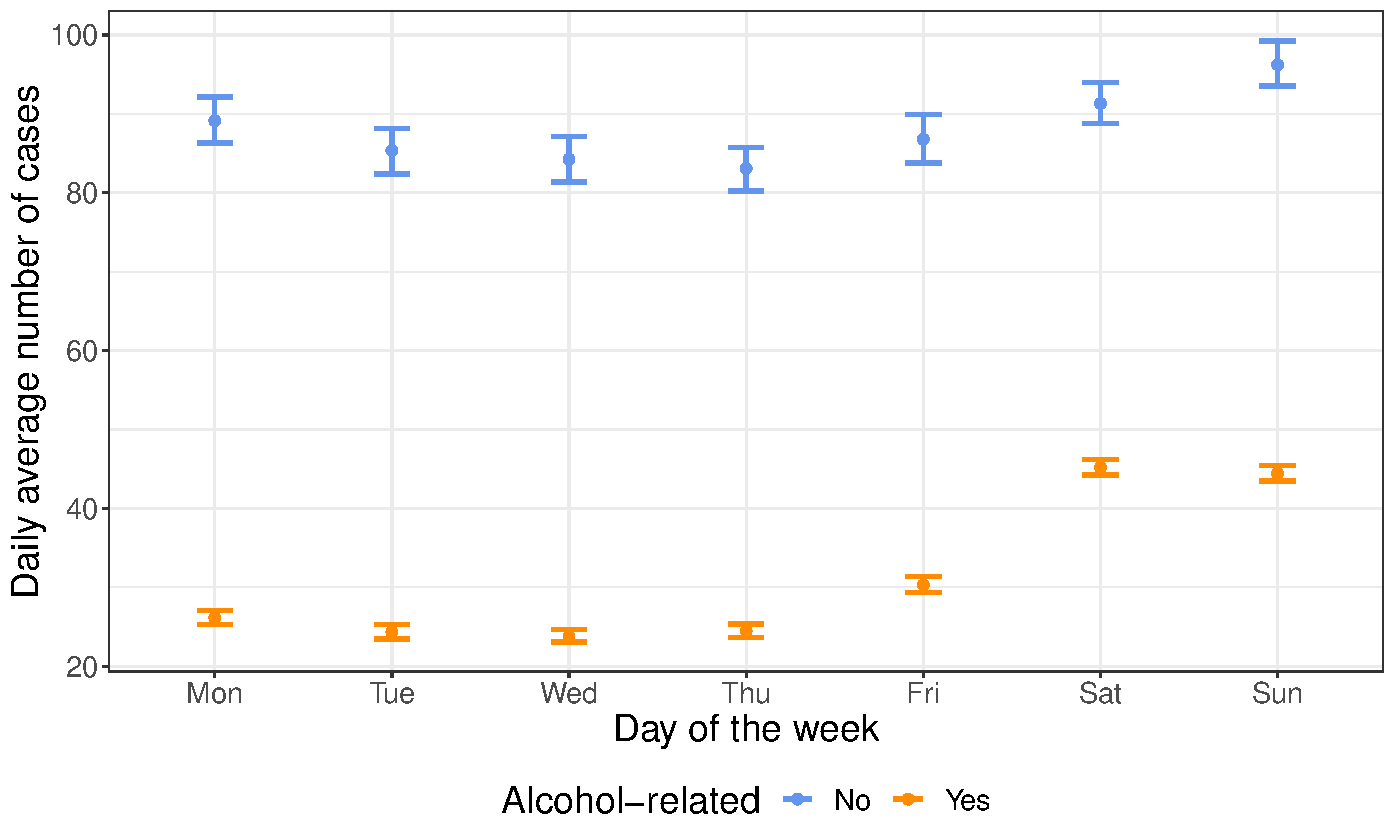
\includegraphics[scale = 0.6]{descriptives.pdf}
\caption{The daily average number of alcohol and non-alcohol related domestic abuse cases reported to the police, by day of the week. The error bars show bootstrapped 95\% confidence intervals, stratified by month. \label{fig:descriptive}} 
\end{center} 
\end{figure} 

In the UK, the term ``domestic abuse'' refers to a wide range of behavioural patterns, from physical and sexual violence to psychological, emotional, financial abuse, threatening behaviour, stalking and harassment, either within a family or an intimate relationship \cite{ONS}. Previous research has mostly focused on intimate partner violence (IPV), the largest subcategory of domestic abuse. While IPV is more common than abuse perpetrated by family members \cite{ONS}, our dataset does not contain information about the exact relationship between the victim and perpetrator (family vs current or ex-partner), therefore we cannot separate the two types of abuse, and we will refer to them collectively as ``domestic abuse''.


Our dataset contains all cases of domestic abuse that have been reported to the WMP between 2010 and 2019, but the vast majority of domestic abuse incidents in fact never get reported (according to the Crime Survey of England and Wales, only 17\% of domestic abuse victims reported the abuse to the police between April 2017 and March 2018; \citeNP{ONS}). This substantial reporting bias, and its potential correlation with other contextual factors warrants a careful interpretation of the estimates from any quantitative study investigating domestic abuse, and highlights the importance of utilising a mixed methods approach to explore the factors contributing to the prevalence of domestic abuse. 
  
 
 
\begin{table}[!htbp]
\centering
    \caption{Matches of the English national football team in the World Cup and European Championship tournaments between 2010 and 2019, by outcome.}
\begin{tabular}{ccccc}
  \hline
\textbf{Date} & \textbf{Other Team} & \textbf{Tournament} & \textbf{Year} & \textbf{Outcome} \\ 
  \hline
2010-06-12 & USA & World Cup & 2010 & England draw \\ 
  2010-06-18 & Algeria & World Cup & 2010 & England draw \\ 
  2010-06-23 & Slovenia & World Cup & 2010 & England win \\ 
  2010-06-27 & Germany & World Cup & 2010 & England lost \\ 
  2012-06-11 & France & European Championship & 2012 & England draw \\ 
  2012-06-15 & Sweden & European Championship & 2012 & England win \\ 
  2012-06-19 & Ukraine & European Championship & 2012 & England win \\ 
  2012-06-24 & Italy & European Championship & 2012 & England lost \\ 
  2014-06-14 & Italy & World Cup & 2014 & England lost \\ 
  2014-06-19 & Uruguay & World Cup & 2014 & England lost \\ 
  2014-06-24 & Costa Rica & World Cup & 2014 & England draw \\ 
  2016-06-11 & Russia & European Championship & 2016 & England draw \\ 
  2016-06-16 & Wales & European Championship & 2016 & England win \\ 
  2016-06-20 & Slovakia & European Championship & 2016 & England draw \\ 
  2016-06-27 & Iceland & European Championship & 2016 & England lost \\ 
  2018-06-18 & Tunisia & World Cup & 2018 & England win \\ 
  2018-06-24 & Panama & World Cup & 2018 & England win \\ 
  2018-06-28 & Belgium & World Cup & 2018 & England lost \\ 
  2018-07-03 & Colombia & World Cup & 2018 & England win \\ 
  2018-07-07 & Sweden & World Cup & 2018 & England win \\ 
  2018-07-11 & Croatia & World Cup & 2018 & England lost \\ 
  2018-07-14 & Belgium & World Cup & 2018 & England lost \\ 
   \hline
\end{tabular}
  \label{Tab:matches}
\end{table}

 There were three World Cups (2010, 2014, 2018) and two European Championships (2012, 2016) in the period covered by our dataset. All of these tournaments took place in the months of June and July. 
Table \ref{Tab:matches} shows the matches of the English national football team in these tournaments. Out of 22 matches overall, England won and lost both eight times, while six matches ended in a draw. 

\section{Methods}

To investigate the role alcohol plays in the link between England football matches and domestic abuse, we used a regression framework. Our main results are derived from Poisson and Negative Binomial regressions, where each observation is a day or a three-hour interval in the period between 2010 and 2019, and the outcome variable is the number of cases perpetrated in an observation period. To investigate certain characteristics of the domestic abuse cases perpetrated on England match days, we also used a logistic regression framework. Below is a detailed explanation of the statistical models used in our analyses.  


\subsection{Count per day analyses} 
\label{modelsexplained}


In these regressions, each day in our dataset is an observation (of which there are 3570), and the outcome variable is the number of domestic abuse cases perpetrated on that day (alcohol-related or not). We classified each day in this period as one of the following: England won (England win, $N = 8$), lost (England lost, $N = 8$) or drew (England draw, $N = 6$), a day after an England match day (After England, $N = 22$), any other day during the months of the tournament (Tournament on, $N = 106$), or any other day during the rest of the year (Non-match day, $N = 3420$). Our aim is to understand the extent to which this classification variable can explain the number of alcohol-related and non-alcohol related cases reported to the police.

To control for potential confounders and account for the temporal variability of the number of domestic abuse cases, we also added a set of dummy  variables, including day of the week, calendar month, and year. 
We included a dummy for Christmas cases (covering the period between 24th and 26th of December) and New Year's Eve cases (in the early morning of 1st of January). 
These holidays are consistently associated with an increased number of domestic abuse cases reported to the police, therefore including these will result in a more precise estimate of the association between football and domestic abuse.

Given that our outcome variable is a count, we considered using a Poisson or a negative binomial regression model framework. 
Formally, if $C_i$ is the number of reported cases (alcohol or non-alcohol related) on days $i = 1...N$, then these models can be formally expressed as
%
\begin{equation}
 \ln(\lambda_i) =\vect{x_i^{T}}\vect{\beta}
\end{equation}


where 
$C_i \sim Pois(\lambda_i)$ or $C_i \sim Negative Binomial(\lambda_i,\theta)$, $\vect{x_i}$, is a vector of covariates, and $\boldsymbol{\beta}$ is the vector of coefficients.

In the Poisson framework, it is assumed that the mean of the distribution ($\lambda_i$) is equal to the variance. 
However, for certain types of count data, the observed variance can exceed the mean, causing overdispersion. 
If overdispersion is present in the data, the Poisson model understates the standard error of the estimates, leading to erroneous conclusions. 
Given the complex nature of domestic abuse, it is likely that our model will not able to fully account for all the factors influencing the number of reported cases on a given day, leading to unobserved heterogeneity and increasing the likelihood of overdispersion. 
Testing for overdispersion in a Poisson model involves testing the null-hypothesis of equidispersion (the mean being equal to the variance).
If there is evidence for overdispersion, a negative binomial model is a more suitable modelling framework, as it includes an additional parameter $\theta$ to allow the variance to deviate from the mean. 


\subsection{Count per three-hour interval analysis}

In this analysis, we used the regression framework described in section \ref{modelsexplained} (either Poisson or negative binomial regression) to investigate the temporal dynamics of the number of domestic abuse cases (alcohol-related or not) perpetrated before and after England matches. To this end, we divided each day in our dataset into eight three-hour periods, the first one starting at 12am, and used these to identify specific time windows around the time of the match (six and three hours before the match, during match, and three, six, twelve, and twenty-four hours after the match). The exact time of the matches vary considerably (the earliest starting at 1pm, and the latest at 11pm). We first identified the three-hour period of the day into which each match falls. If the start and end time of the match did not fall in the same three-hour period, we chose the three-hour period that covers the larger part of the match (e.g., a 2.5 hour long match starting at 7pm will be assigned to the 6-9pm period and not to the 9pm-12am period). In these regressions, each time window indicator is a dummy variable, therefore the exponentiated coefficients directly represent the relative change in the number of cases during these periods, compared to any other (overwhelmingly non-match) periods. To control for potential confounders, we controlled for year, month, day of week, three-hour period of the day, Christmas and New Year's Eve.


\subsection{Binary outcome variable analyses}

To further understand the characteristics of domestic abuse cases perpetrated on England football days, such as whether these cases are more likely to occur in a public location or end in serious injury, we used a logistic regression framework. 
Given a binary response variable ($Y_{i}$ can either take the value 0 or 1), we wish to model the probability of an event occurring, i.e., $\pi = P(Y = 1)$. 
In a logistic regression framework, we can model this probability with the equation

\begin{equation}
log(\frac{\pi}{1-\pi})= \vect{x_i^{T}}\vect{\beta}
\end{equation}

where \textbf{x\textsubscript{i}} is a vector of covariates, and $\boldsymbol{\beta}$ is the vector of coefficients.


\newpage

\section{Results}

In the following count data analyses, we present results from negative binomial models, as we found evidence for overdispersion in all cases (after testing for overdispersion using the method described in \citeNP{Cameron1990a}). All analyses were performed in R (version 3.6.2).


\subsection{Core results} 

Table \ref{coremodel} shows the results from two negative binomial regressions investigating the link between football and domestic abuse, one for non-alcohol-related cases and one for alcohol-related cases. For non-alcohol-related cases, we find no evidence for an increase (or decrease) on days when the England football team plays, compared to non-match days. In contrast, we see a significant, 47\%, 95\% CI [26\%--71\%], increase in the number of alcohol-related cases on days when the England football team wins, compared to non-match days. We find no evidence for comparable increases in the number of reported domestic abuse cases when the England national team loses. Less surprising, and more consistent with previous findings is the lack of evidence for an increase on England draw days, probably due to the fact that high-stake matches after the group-stage in the tournament cannot result in a draw. In addition, we estimate that there is an 18\%, 95\% CI [7\%--30\%], increase in the number of alcohol-related cases reported after an England match day, which could be the result of a temporal spill-over effect from the previous match day. 


\begin{table*}[!htbp] \centering 
  \begin{threeparttable}
  \caption{The effect of England football days on domestic abuse by alcohol-involvement, 2010-2019} 
  \label{coremodel} 
\begin{tabular}{@{\extracolsep{5pt}}lcc} 
\\[-1.8ex]\hline 
\hline \\[-1.8ex] 
 & \multicolumn{2}{c}{\textit{Dependent variable:}} \\ 
\cline{2-3} 
\\[-1.8ex] & \multicolumn{2}{c}{Number of cases} \\ 
 & Non-alcohol related & Alcohol-related\\ 
 & domestic abuse & domestic abuse\\
\\[-1.8ex] & (1) & (2)\\ 
%\hline \\[-1.8ex] 
\hline \\[-1.8ex] 
 Tournament on & 1.024 & 0.984 \\ 
  & (0.986, 1.064) & (0.935, 1.037) \\ 
  %& & \\ 
 England win & 0.950 & 1.469$^{***}$ \\ 
  & (0.838, 1.077) & (1.259, 1.714) \\ 
  %& & \\ 
 England draw & 1.045 & 1.145 \\ 
  & (0.905, 1.208) & (0.955, 1.375) \\ 
  %& & \\ 
 England lost & 1.033 & 1.129 \\ 
  & (0.915, 1.167) & (0.963, 1.324) \\ 
  %& & \\ 
 After England & 1.056 & 1.181$^{***}$ \\ 
  & (0.979, 1.140) & (1.069, 1.305) \\ 
  %& & \\ 
\hline \\[-1.8ex] 
Observations & 3,570 & 3,570 \\ 
%Log Likelihood & $-$14,692.790 & $-$12,071.110 \\ 
%$\theta$ & 51.259$^{***}$  (1.967) & 39.423$^{***}$  (2.112) \\ 
%Akaike Inf. Crit. & 29,453.580 & 24,210.210 \\ 
\hline 
\hline \\[-1.8ex] 
Notes:
%\textit{Note:}  & \multicolumn{2}{r}{$^{*}$p$<$0.1; $^{**}$p$<$0.05; $^{***}$p$<$0.01} \\ 
\end{tabular} 
\begin{tablenotes}
      \item[a] \textit{$^{*}$p$<$0.1; $^{**}$p$<$0.05; $^{***}$p$<$0.01}
      \item[b] \textit{Estimates are exponentiated coefficients from negative binomial regressions with non-match day as benchmark; controls include day of week, month, year, Christmas, and New Year's Eve}
    \end{tablenotes}
\end{threeparttable} 
\end{table*}







 \begin{figure}[!htbp]
\centering
 \caption{The temporal dynamics of the number of domestic abuse cases perpetrated on England draw, lose, and win days, by alcohol involvement.}
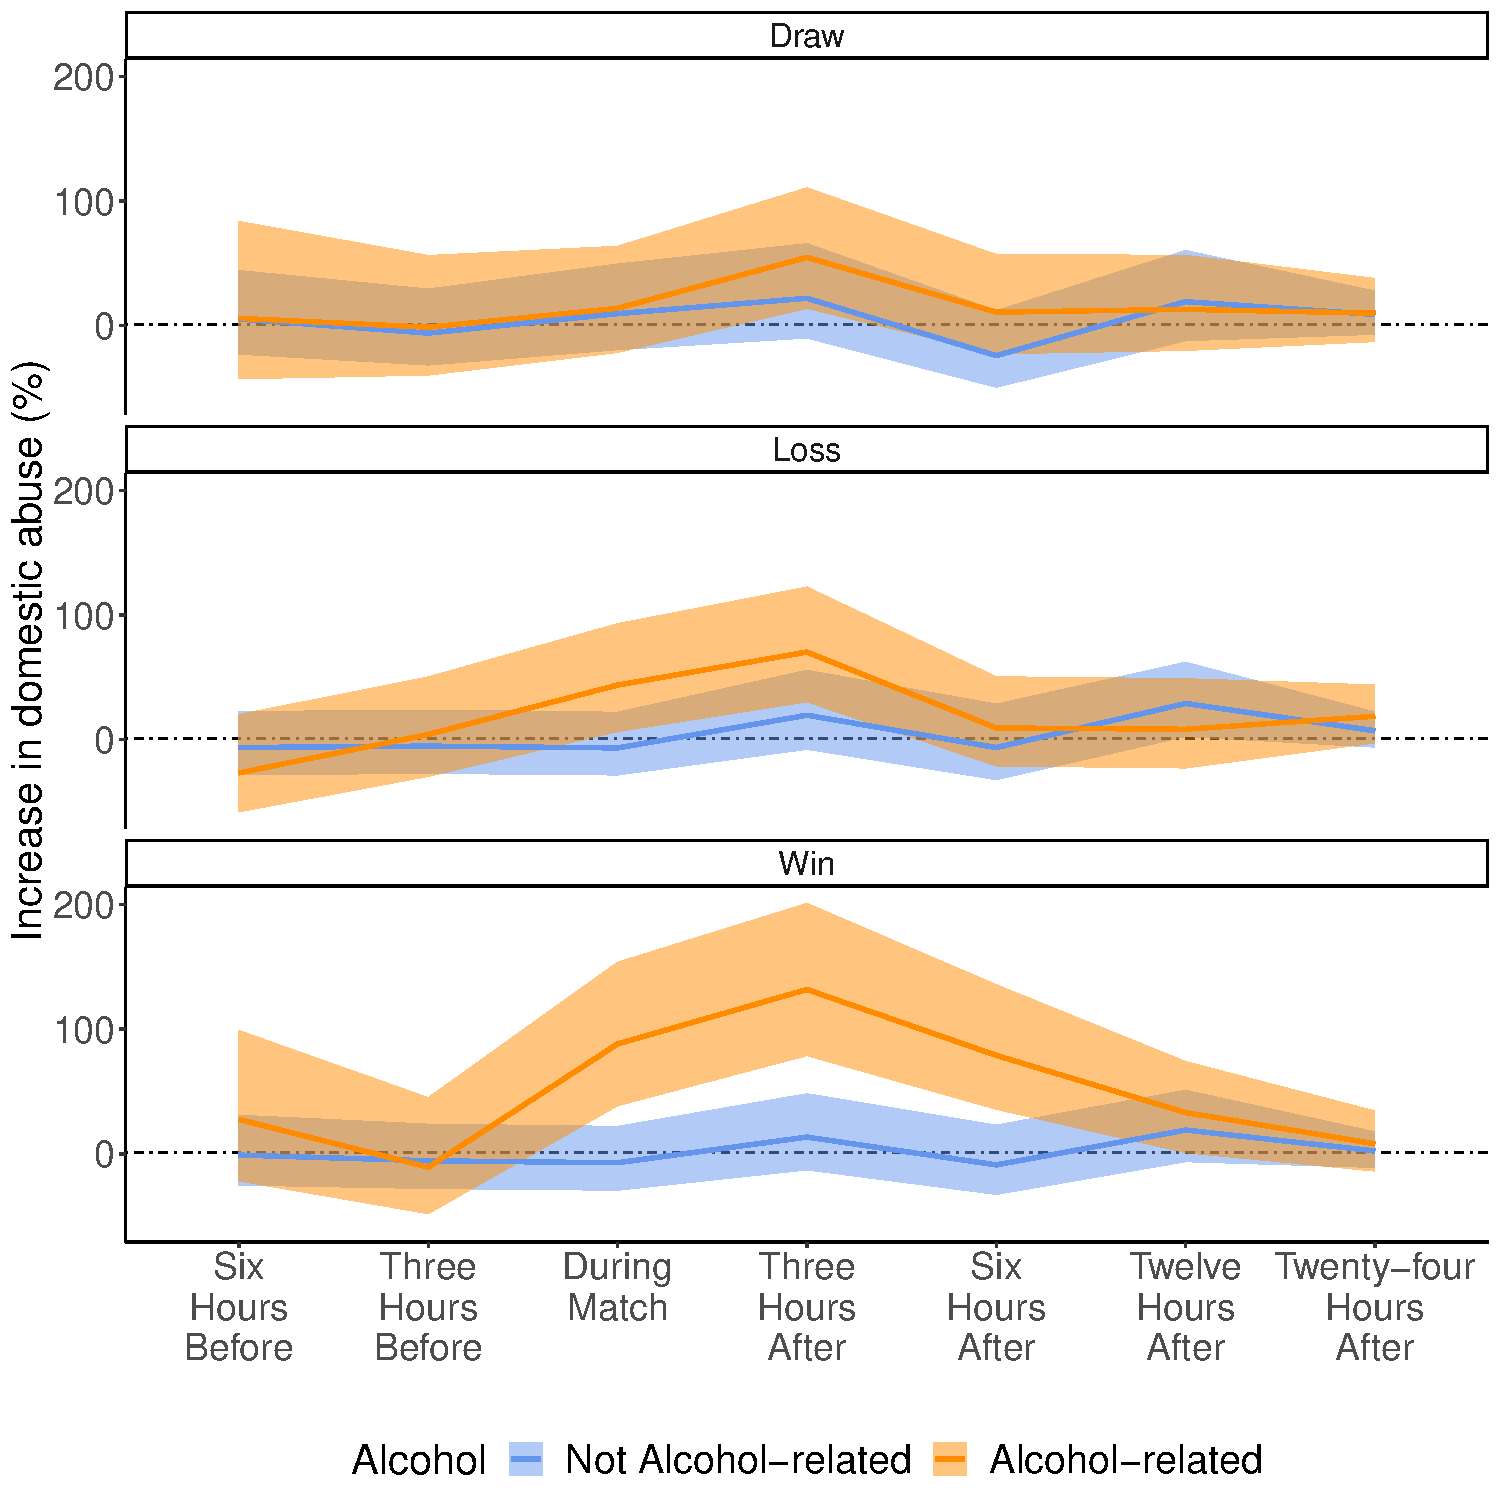
\includegraphics[width=0.75\textwidth]{Threehours_newdata.pdf}
\label{fig:threehours}
		\floatfoot{Note: Estimates are from two separate negative binomial regressions with year, month, day of week, three-hour period of day, Christmas, New Year's eve controls. Shaded area is 95\% CIs.}
\end{figure}

 To further understand the characteristics of this increase, we exploited the detailed time information in our dataset, which allowed us to conduct a three-hour analysis to explore the finer temporal patterns of domestic abuse cases (alcohol-related or not) perpetrated before and after an England match. Figure \ref{fig:threehours} shows a plot of the estimated percentage increase from these negative binomial regressions, revealing a stark increase in alcohol-related domestic abuse on days of an England victory, starting in the three hour period of the match, peaking in the three-hour period afterwards, and gradually declining to its original level in the twenty-four hours following the victory. While a similar pattern can be observed on days when England lost, the increase in the number of alcohol-related cases is substantially smaller and not statistically different from zero.

\subsection{Other types of crimes and incidents}

Our crime dataset further allows us to explore whether England games have similar effects on other types of criminal behaviours, apart from domestic abuse. Specifically, we are interested in how an England match day affects the number of reported property-related crimes (where the offence class is either theft or robbery), hate crimes (where the offence description includes the words ``hate'', ``racial'' or ``racially''), and other violent crimes (where the offence class is classified as violence against the person, after excluding cases of domestic abuse). Of particular interest is the effect of football on non-domestic violent crimes, since it is possible that alcohol-fuelled violence that follows an England victory is not limited to family and intimate partner relationships. 

\AT{I think we should say something about how detecting alcohol-involvement varies by crime type- e.g., for domestic abuse we have greater confidence in identifying alcohol-related cases as opposed to property-related crimes}


Table \ref{othercrimes} shows the results for these three types of criminal behaviours, by alcohol-involvement. Compared to non-match days, hate crimes and incidents with no alcohol-involvement increase by 12\%, 95\% CI [3\%--22\%], during the months of the tournaments. Similarly, compared to non-match days, alcohol-related thefts and robberies (property-related offences) increase by 10\%, 95\% CI [1\%--19\%], when the tournament is on, and by 29\%, 95\% CI [0\%--66\%] \NS{CI in table extends just below 1, so how is this significant at 5\% level?}, when England wins, although these estimates are not very precise (demonstrated by the width of the confidence intervals), due to the relatively small number of alcohol-related theft and robbery cases. In contrast, the effect of an England win on alcohol-related cases clearly extends to other, non-domestic violent offences, resulting in a 47\%, 95\% CI [19\%--83\%], increase compared to non-match days. While it is possible that misclassified domestic abuse cases contribute to this result (e.g, if the victim chooses not to disclose any relationship to the offender), these results suggests that the increase in alcohol-related violence following an England victory is not limited to domestic settings. \NS{What happened to the analysis showing that this was especially true for male-to-female abuse?}



  \begin{sidewaystable}[htp]
\centering
 \caption{The effect of England football days on hate-related, property-related, and other violent offences by alcohol-involvement}
   \label{othercrimes}
    \scalebox{0.9}{
 \begin{threeparttable}
\begin{tabular}{@{\extracolsep{1pt}}lcccccc} 
\\[-1.8ex]\hline 
\hline \\[-1.8ex] 
 & \multicolumn{6}{c}{\textit{Dependent variable:}} \\ 
   & \multicolumn{6}{c}{Number of cases} \\ 
  & \multicolumn{3}{c}{Non-alcohol related} &\multicolumn{3}{c}{Alcohol-related} \\
\cline{2-7} 
\\[-1.8ex] & Hate- & Property- & Other & Hate- & Property & Other \\ & related & related & violent & related & related & violent \\ 
\\[-1.8ex] & (1) & (2) & (3) & (4) & (5) & (6)\\ 
\hline \\[-1.8ex] 
Tournament & 1.120$^{***}$ & 1.014 & 1.035 & 1.099 & 1.099$^{**}$ & 1.060 \\ 
 on & (1.030, 1.216) & (0.986, 1.043) & (0.986, 1.085) & (0.914, 1.316) & (1.011, 1.194) & (0.987, 1.139) \\ 
  & & & & & & \\ 
England & 1.002 & 0.961 & 1.085 & 1.556$^{*}$ & 1.291$^{**}$ & 1.473$^{***}$ \\ 
win & (0.759, 1.311) & (0.879, 1.052) & (0.935, 1.263) & (0.902, 2.558) & (0.998, 1.662) & (1.192, 1.826) \\ 
  & & & & & & \\ 
England & 0.993 & 0.953 & 0.970 & 0.848 & 0.934 & 1.251$^{*}$ \\ 
 draw & (0.709, 1.369) & (0.859, 1.059) & (0.810, 1.167) & (0.400, 1.624) & (0.701, 1.237) & (0.974, 1.613) \\ 
  & & & & & & \\ 
England & 0.984 & 0.974 & 1.066 & 0.760 & 1.008 & 0.988 \\ 
 lost & (0.744, 1.288) & (0.890, 1.066) & (0.917, 1.243) & (0.363, 1.427) & (0.744, 1.353) & (0.785, 1.247) \\ 
  & & & & & & \\ 
After & 1.124 & 0.978 & 1.085$^{*}$ & 1.244 & 1.047 & 1.092 \\ 
 England & (0.953, 1.323) & (0.925, 1.035) & (0.988, 1.193) & (0.872, 1.742) & (0.884, 1.237) & (0.948, 1.258) \\ 
  & & & & & & \\ 
\hline \\[-1.8ex] 
Observations & 3,570 & 3,570 & 3,570 & 3,570 & 3,570 & 3,570 \\ 
%Log Likelihood & $-$9,086.944 & $-$15,273.310 & $-$14,697.050 & $-$5,347.670 & $-$8,646.912 & $-$11,171.590 \\ 
%$\theta$ & 23.936$^{***}$  (2.255) & 110.360$^{***}$  (4.838) & 29.145$^{***}$  (0.972) & 9.774$^{***}$  (1.829) & 30.885$^{***}$  (3.014) & 18.765$^{***}$  (0.926) \\ 
%Akaike Inf. Crit. & 18,241.890 & 30,614.620 & 29,462.100 & 10,763.340 & 17,361.830 & 22,411.180 \\ 
\hline 
\hline \\[-1.8ex] 
\textit{Note:}  & \multicolumn{6}{r}{$^{*}$p$<$0.1; $^{**}$p$<$0.05; $^{***}$p$<$0.01} \\ 
\end{tabular} 
\begin{tablenotes}
      \item[a] \textit{$^{*}$p$<$0.1; $^{**}$p$<$0.05; $^{***}$p$<$0.01}
      \item[b] \textit{Estimates are exponentiated coefficients from a series of negative binomial regressions with non-match day as benchmark; controls include day of week, month, year, Christmas, and New Year's Eve}
    \end{tablenotes}
\end{threeparttable} }
\end{sidewaystable}

\subsection{Other types of sports: rugby}
Does this effect generalise to other sporting events, or is it specific to football? It has been previously suggested that other popular sports, such as rugby have similar links with domestic abuse \cite{Brooks-Hay2018}. Rugby is the second most popular sport in England after football \cite{Ipsos2003}. Focusing on the Six Nations, a high-profile rugby tournament that takes place every year in the months of February and March with the participation of England, Wales, Scotland, Ireland, France and Italy, we explored whether the reported number of domestic abuse cases increase on days when the England national rugby team plays. 

Each tournament year, England plays one match with each of the other five participating countries, and these matches take place almost always during the weekend (Saturday, $N = 37$; Sunday, $N = 11$; Friday, $N = 2$). The most common result for England is to win ($N = 35$), much less frequent are losses ($N = 12$), and draws ($N = 2$).


Table \ref{rugby} shows no comparable effects for rugby matches on domestic abuse, potentially stemming from differences in timing, media coverage, audience numbers, and the involvement of alcohol between the two tournaments. \TM{Do we want to cite socioeconomic and sociodemographic differences? i.e. Rugby fans are rich and posh.}


\begin{table*}[!htbp] \centering 
  \begin{threeparttable}
  \caption{The effect of England rugby days (Six Nations) on domestic abuse by alcohol-involvement} 
  \label{rugby} 
\begin{tabular}{@{\extracolsep{5pt}}lcc} 
\\[-1.8ex]\hline 
\hline \\[-1.8ex] 
 & \multicolumn{2}{c}{\textit{Dependent variable:}} \\ 
\cline{2-3} 
\\[-1.8ex] & \multicolumn{2}{c}{Number of cases} \\ 
 & Non-alcohol related & Alcohol-related\\ 
 & domestic abuse & domestic abuse\\
\\[-1.8ex] & (1) & (2)\\ 
\hline \\[-1.8ex] 
 Tournament on & 0.980 & 0.969 \\ 
  & (0.947, 1.014) & (0.923, 1.017) \\ 
 % & & \\ 
 England win & 0.967 & 1.058 \\ 
  & (0.906, 1.033) & (0.973, 1.151) \\ 
 % & & \\ 
 England draw & 1.030 & 0.966 \\ 
  & (0.810, 1.318) & (0.716, 1.308) \\ 
 % & & \\ 
 England lost & 1.067 & 0.989 \\ 
  & (0.963, 1.184) & (0.867, 1.129) \\ 
 % & & \\ 
 After England & 0.983 & 1.004 \\ 
  & (0.929, 1.041) & (0.931, 1.083) \\ 
 % & & \\ 
\hline \\[-1.8ex] 
Observations & 3,570 & 3,570 \\ 
%Log Likelihood & $-$14,692.860 & $-$12,087.270 \\ 
%$\theta$ & 51.260$^{***}$  (1.967) & 38.539$^{***}$  (2.040) \\ 
%Akaike Inf. Crit. & 29,453.730 & 24,242.540 \\ 
\hline 
\hline \\[-1.8ex] 
Notes:
%\textit{Note:}  & \multicolumn{2}{r}{$^{*}$p$<$0.1; $^{**}$p$<$0.05; $^{***}$p$<$0.01} \\ 
\end{tabular} 
\begin{tablenotes}
      \item[a] \textit{$^{*}$p$<$0.1; $^{**}$p$<$0.05; $^{***}$p$<$0.01}
      \item[b] \textit{Estimates are exponentiated coefficients from negative binomial regressions with non-match day as benchmark; controls include day of week, month, year, Christmas, and New Year's Eve}
    \end{tablenotes}
\end{threeparttable} 
\end{table*}

\FloatBarrier


\subsection{Previous evidence}


A previous study by \citeA{Kirby2014} found that an England loss results in the most pronounced increase in domestic abuse (38\%), and a win or draw have a slightly smaller effect (26\%). They used daily counts of IPV in Lancashire from the months of the 2002, 2006, 2010 World Cups. Upon re-analysing their data by treating wins and draws as two separate variables (see Table \ref{kirbyrep1}), we see a roughly similar effect for wins (45\%, 95\% CI [28\%--64\%]) and losses (39\%, 95\% CI [18\%--64\%]), and no effect when England draws. Separating wins and draws clearly improves the fit of the model, demonstrated by the reduction in the Bayesian and Akaike Information Criteria (BIC and AIC, respectively). However, the estimated effect of an England loss is insensitive to this change. In conclusion, our reanalysis replicates the win effect seen in the West Midlands data, though the absence of a loss effect remains a difference between the two studies.

\begin{table*}[!htb]
\centering
 \caption{Re-analysis of Kirby et al. (2014) with wins and draws as separate variables}
   \label{kirbyrep1}
   \scalebox{0.85}{
 \begin{threeparttable}
\begin{tabular}{@{\extracolsep{5pt}}lcc} 
\\[-1.8ex]\hline 
\hline \\[-1.8ex] 
 & \multicolumn{2}{c}{\textit{Dependent variable:}} \\ 
\cline{2-3} 
\\[-1.8ex] & \multicolumn{2}{c}{Number of reported Intimate Partner Violence cases per day} \\ 
\\ 
  & Original Model & Win/Draw Separate \\ 
\\[-1.8ex] & (1) & (2)\\ 
\hline \\[-1.8ex] 
 England windraw & 1.256$^{***}$ &  \\ 
  & (1.128, 1.398) &  \\ 
  England lost & 1.382$^{***}$ & 1.388$^{***}$ \\ 
  & (1.151, 1.662) & (1.175, 1.639) \\ 
  After England & 1.111$^{**}$ & 1.113$^{**}$ \\ 
  & (1.004, 1.228) & (1.014, 1.221) \\ 
  England win &  & 1.452$^{***}$ \\ 
  &  & (1.282, 1.644) \\ 
  England draw &  & 1.032 \\ 
  &  & (0.893, 1.191) \\ 
%  England lost &  & 1.388$^{***}$ \\ 
%  &  & (1.175, 1.639) \\ 
%  After England &  & 1.113$^{**}$ \\ 
%  &  & (1.014, 1.221) \\ 
 \hline \\[-1.8ex] 
Observations & 92 & 92 \\ 
BIC & 747.763 & 739.662 \\ 
AIC & 714.980 & 704.356 \\ 
\hline 
\hline \\[-1.8ex] 
\end{tabular} 
\begin{tablenotes}
      \item[a] \textit{$^{*}$p$<$0.1; $^{**}$p$<$0.05; $^{***}$p$<$0.01}
      \item[b] \textit{Estimates are exponentiated coefficients from negative binomial regressions (based on tests of overdispersion) with year and day of week controls and no England match days during the tournament as benchmark; data is only available during the tournament period}
    \end{tablenotes}
\end{threeparttable} }
\end{table*}


To explore the underlying reason for this discrepancy and test the robustness of our results, we find it instructive to break our analysis into specific tournament years (Lancashire and West Midlands; see Table \ref{kirbyrep2}). To be consistent with previous results, we present the regressions for both types of domestic abuse (alcohol and non-alcohol related), however, unfortunately we cannot do the same for the Lancashire dataset, as we have no information on alcohol-involvement. Only year 2010 overlaps in the two datasets, which allows us to at least partly evaluate the robustness of the England win effect.

An interesting common pattern in both datasets is the large effect of England's victory over Slovenia in the group stage of the 2010 World Cup, which, after much anticipation, secured their progression to the next stage of the tournament. Equally, the subsequent loss against Germany in the knockout stage resulted in a substantial increase in the number of reported domestic abuse incidents, which is the strongest loss effect in our dataset. In addition, the size of the win and loss coefficients are remarkably similar, giving us confidence that these effects are likely to generalise to other areas within England. These patterns are also in line with findings from an earlier examination by \cite{Brimicombe2012}, who found an increase in the number of domestic abuse cases reported to the police across England on both victory and loss days during the 2010 World Cup.  Most importantly, if the same mechanism lies behind our results, then it suggests that the increase observed in other datasets are also likely to stem from alcohol-related cases. 
   
  It's also clear that World Cup wins have the strongest effect on the number of domestic abuse incidents: a clear, large increase can be observed in 2002, 2006, 2010, and 2018 (England did not have a single victory in the 2014 World Cup). The number of domestic abuse cases also increase after England losses in World Cup tournament years, but this effect is usually about half the size of the win effect (except for 2006).
  
  As a further robustness check, we examine the sensitivity of the result to the exclusion of specific tournament years  (see Table \ref{robustness}). This analysis shows that while the size of the England win effect varies by year, it is robust to the exclusion of specific tournament years, and is not driven by an unusually large effect in one of the tournament years.

%\newpage



\begin{sidewaystable}[htp]
\centering
 \caption{The effect of England football days on domestic abuse by alcohol-involvement and tournament, Lancashire and West Midlands data}
   \label{kirbyrep2}
    \scalebox{0.65}{
 \begin{threeparttable}
\begin{tabular}{@{\extracolsep{1pt}}lccccccccccccc} 
\\[-1.8ex]\hline 
\hline \\[-1.8ex] 
 & \multicolumn{13}{c}{\textit{Dependent variable:}} \\ 
\cline{2-14} 
& \multicolumn{13}{c}{Number of domestic abuse cases} \\ 
\\[-1.8ex] & \multicolumn{3}{c}{Lancashire} & \multicolumn{10}{c}{West Midlands} \\ 
\\[-1.8ex] & \multicolumn{1}{c}{All\textsuperscript{c}} & \multicolumn{1}{c}{All} & \multicolumn{1}{c}{All} & \multicolumn{1}{c}{NA\textsuperscript{c}} & \multicolumn{1}{c}{A\textsuperscript{c}} & \multicolumn{1}{c}{NA} & \multicolumn{1}{c}{A} & \multicolumn{1}{c}{NA} & \multicolumn{1}{c}{A} & \multicolumn{1}{c}{NA} & \multicolumn{1}{c}{A} & \multicolumn{1}{c}{NA} & \multicolumn{1}{c}{A} \\ 
% & \textit{binomial} & \multicolumn{2}{c}{\textit{}} & \multicolumn{10}{c}{\textit{binomial}} \\ 
 \\[-1.8ex] & 2002 & 2006 & 2010 & 2010 & 2010 & 2012 & 2012 & 2014 & 2014 & 2016 & 2016 & 2018 & 2018  \\ 
\\[-1.8ex] & (1) & (2) & (3) & (4) & (5) & (6) & (7) & (8) & (9) & (10) & (11) & (12) & (13)\\ 
\hline \\[-1.8ex] 
 Tournament on &  &  &  & 1.047 & 1.038 & 0.881 & 0.936 & 0.976 & 0.999 & 1.041 & 0.855$^{**}$ & 1.081 & 1.014 \\ 
  &  &  &  & (0.974, 1.127) & (0.936, 1.151) & (0.740, 1.049) & (0.780, 1.125) & (0.901, 1.057) & (0.890, 1.123) & (0.962, 1.128) & (0.757, 0.967) & (0.979, 1.194) & (0.889, 1.155) \\ 
  England win & 1.596$^{***}$ & 1.297$^{***}$ & 1.916$^{***}$ & 1.171 & 1.845$^{***}$ & 0.673$^{**}$ & 1.106 &  &  & 1.062 & 1.302 & 1.006 & 1.529$^{***}$ \\ 
  & (1.186, 2.153) & (1.115, 1.505) & (1.528, 2.389) & (0.897, 1.514) & (1.310, 2.595) & (0.456, 0.982) & (0.770, 1.576) &  &  & (0.796, 1.420) & (0.834, 1.995) & (0.844, 1.202) & (1.249, 1.869) \\ 
 England draw & 1.100 & 1.098 & 0.863 & 0.905 & 1.248$^{*}$ & 1.204 & 1.116 & 0.984 & 0.954 & 1.069 & 1.128 &  &  \\ 
  & (0.820, 1.477) & (0.802, 1.481) & (0.713, 1.037) & (0.736, 1.107) & (0.966, 1.611) & (0.773, 1.877) & (0.676, 1.805) & (0.723, 1.343) & (0.576, 1.527) & (0.869, 1.318) & (0.835, 1.517) &  &  \\ 
 England lost & 1.200 & 1.373$^{***}$ & 1.568$^{***}$ & 1.082 & 1.435$^{**}$ & 0.812 & 0.961 & 0.934 & 1.079 & 0.772$^{*}$ & 0.620$^{*}$ & 1.101 & 1.252$^{*}$ \\ 
  & (0.759, 1.894) & (1.086, 1.721) & (1.270, 1.928) & (0.838, 1.389) & (1.036, 1.992) & (0.508, 1.293) & (0.614, 1.491) & (0.747, 1.170) & (0.792, 1.459) & (0.568, 1.048) & (0.343, 1.058) & (0.904, 1.348) & (0.975, 1.603) \\ 
 After England & 1.253$^{**}$ & 1.122$^{*}$ & 1.024 & 1.049 & 1.132 & 0.814 & 1.108 & 1.037 & 1.080 & 1.013 & 0.960 & 1.147$^{*}$ & 1.390$^{***}$ \\ 
  & (1.029, 1.526) & (0.977, 1.286) & (0.900, 1.162) & (0.905, 1.194) & (0.933, 1.331) & (0.535, 1.092) & (0.834, 1.381) & (0.863, 1.249) & (0.832, 1.394) & (0.853, 1.172) & (0.715, 1.206) & (1.001, 1.317) & (1.173, 1.646) \\ 
 \hline \\[-1.8ex] 
Observations & 30 & 32 & 30 & 365 & 365 & 366 & 366 & 365 & 365 & 366 & 366 & 365 & 365 \\ 
%Log Likelihood & $-$112.494 & $-$101.847 & $-$107.268 & $-$1,344.208 & $-$1,305.710 & $-$1,294.898 & $-$1,189.726 & $-$1,494.583 & $-$1,175.810 & $-$1,503.841 & $-$1,197.151 & $-$1,594.487 & $-$1,200.743 \\ 
%$\theta$ & 57.581$^{*}$  (31.978) &  &  & 215.538$^{***}$  (65.249) & 76.028$^{***}$  (16.053) & 43.908$^{***}$  (6.783) & 55.674$^{***}$  (12.862) & 75.808$^{***}$  (9.733) & 72.582$^{***}$  (18.248) & 90.546$^{***}$  (12.118) & 69.058$^{***}$  (16.506) & 49.787$^{***}$  (5.114) & 64.954$^{***}$  (15.073) \\ 
%Akaike Inf. Crit. & 246.989 & 225.694 & 236.536 & 2,738.415 & 2,661.420 & 2,639.797 & 2,429.452 & 3,037.165 & 2,399.621 & 3,057.682 & 2,444.301 & 3,236.974 & 2,449.485 \\ 
\hline 
\hline \\[-1.8ex] 
\textit{Note:}  & \multicolumn{13}{r}{$^{*}$p$<$0.1; $^{**}$p$<$0.05; $^{***}$p$<$0.01} \\ 
\end{tabular} 
\begin{tablenotes}
      \item[a] \textit{$^{*}$p$<$0.1; $^{**}$p$<$0.05; $^{***}$p$<$0.01}
      \item[b] \textit{Estimates are exponentiated coefficients from a series of negative binomial regressions, except for Model (2) and (3) which are from Poisson regressions (based on tests of overdispersion). Each regression is restricted to a specific tournament year. Regressions 1-3 have day of week control with non England tournament days as benchmark, regressions 4-13 have month, day of week, Christmas, New Year's eve controls, with non-match days as benchmark.}
      \item[c] \textit{All = All cases, NA = Non-alcohol related cases, A = Alcohol-related cases}
    \end{tablenotes}
\end{threeparttable} }
\end{sidewaystable}


\newpage




\begin{sidewaystable}[htp]
\centering
 \caption{Robustness of the result: sensitivity to the exclusion of specific years}
  \label{robustness}
 \scalebox{0.8}{
  \begin{threeparttable}
\begin{tabular}{@{\extracolsep{5pt}}lcccccccccc} 
\\[-1.8ex]\hline 
\hline \\[-1.8ex] 
 & \multicolumn{10}{c}{\textit{Dependent variable:}} \\ 
\cline{2-11} 
\\[-1.8ex] & \multicolumn{10}{c}{Number of domestic abuse cases} \\ 
\\[-1.8ex] & \multicolumn{1}{c}{NA\textsuperscript{c}} & \multicolumn{1}{c}{A\textsuperscript{c}} &  \multicolumn{1}{c}{NA} & \multicolumn{1}{c}{A} &  \multicolumn{1}{c}{NA} & \multicolumn{1}{c}{A} &  \multicolumn{1}{c}{NA} & \multicolumn{1}{c}{A} &  \multicolumn{1}{c}{NA} & \multicolumn{1}{c}{A}  \\
 \\[-1.8ex] & 2010 & 2010 & 2012 & 2012 & 2014 & 2014 & 2016 & 2016 & 2018 & 2018  \\ 
\\[-1.8ex] & (1) & (2) & (3) & (4) & (5) & (6) & (7) & (8) & (9) & (10)\\ 
\hline \\[-1.8ex] 
 Tournament on & 1.035 & 0.959 & 1.063$^{*}$ & 1.084$^{**}$ & 0.976 & 1.085$^{**}$ & 0.960 & 1.105$^{***}$ & 0.948 & 1.069$^{*}$ \\ 
  & (0.946, 1.133) & (0.901, 1.021) & (0.994, 1.136) & (1.014, 1.160) & (0.890, 1.073) & (1.010, 1.166) & (0.877, 1.052) & (1.029, 1.186) & (0.870, 1.034) & (0.997, 1.146) \\ 
  England win & 0.957 & 1.385$^{***}$ & 1.143 & 1.674$^{***}$ & 0.979 & 1.528$^{***}$ & 0.935 & 1.558$^{***}$ & 0.698$^{*}$ & 1.583$^{***}$ \\ 
  & (0.727, 1.289) & (1.154, 1.666) & (0.909, 1.457) & (1.344, 2.100) & (0.753, 1.299) & (1.254, 1.873) & (0.709, 1.262) & (1.262, 1.938) & (0.486, 1.040) & (1.192, 2.127) \\ 
 England draw & 1.037 & 1.126 & 0.990 & 1.347$^{**}$ & 0.921 & 1.383$^{**}$ & 0.793 & 1.391$^{**}$ & 0.950 & 1.304$^{**}$ \\ 
  & (0.724, 1.545) & (0.873, 1.456) & (0.769, 1.297) & (1.056, 1.734) & (0.662, 1.324) & (1.079, 1.788) & (0.550, 1.190) & (1.051, 1.862) & (0.708, 1.306) & (1.034, 1.656) \\ 
  England lost & 1.102 & 1.090 & 1.140 & 1.218$^{*}$ & 1.096 & 1.213 & 1.128 & 1.263$^{**}$ & 0.902 & 1.134 \\ 
  & (0.837, 1.482) & (0.901, 1.322) & (0.922, 1.428) & (0.986, 1.512) & (0.813, 1.520) & (0.964, 1.538) & (0.856, 1.521) & (1.021, 1.574) & (0.655, 1.280) & (0.880, 1.475) \\ 
  After England & 1.095 & 1.198$^{***}$ & 1.169$^{**}$ & 1.287$^{***}$ & 1.054 & 1.283$^{***}$ & 1.043 & 1.316$^{***}$ & 0.891 & 1.205$^{**}$ \\ 
  & (0.914, 1.276) & (1.077, 1.319) & (1.030, 1.307) & (1.151, 1.422) & (0.874, 1.234) & (1.147, 1.418) & (0.860, 1.225) & (1.177, 1.455) & (0.693, 1.088) & (1.050, 1.360) \\ 
 \hline \\[-1.8ex] 
Observations & 3,205 & 3,205 & 3,204 & 3,204 & 3,205 & 3,205 & 3,204 & 3,204 & 3,205 & 3,205 \\ 
%Log Likelihood & $-$15,738.220 & $-$11,006.630 & $-$15,087.610 & $-$11,568.310 & $-$15,673.620 & $-$11,605.220 & $-$15,608.290 & $-$11,602.150 & $-$15,499.280 & $-$11,605.610 \\ 
%$\theta$ & 7.385$^{***}$  (0.199) & 28.051$^{***}$  (1.404) & %13.075$^{***}$  (0.373) & 17.870$^{***}$  (0.723) & 7.139$^{***}$  (0.191) & 16.977$^{***}$  (0.674) & 7.284$^{***}$  (0.196) & 16.694$^{***}$  (0.660) & 7.692$^{***}$  (0.208) & 16.664$^{***}$  (0.658) \\ 
%Akaike Inf. Crit. & 31,526.440 & 22,063.270 & 30,225.220 & 23,186.630 & 31,397.250 & 23,260.450 & 31,266.580 & 23,254.290 & 31,048.560 & 23,261.230 \\ 
\hline 
\hline \\[-1.8ex] 
\textit{Note:}  & \multicolumn{10}{r}{$^{*}$p$<$0.1; $^{**}$p$<$0.05; $^{***}$p$<$0.01} \\ 
\end{tabular} 
%\end{table} 
\begin{tablenotes}
      \item[a] \textit{$^{*}$p$<$0.1; $^{**}$p$<$0.05; $^{***}$p$<$0.01}
      \item[b] \textit{Estimates are exponentiated coefficients from a series of negative binomial regressions (based on tests of overdispersion)  with year, month, day of week, Christmas, New Year's eve controls}
      \item[c] \textit{NA = Non-alcohol related cases, A = Alcohol-related cases}
    \end{tablenotes}
\end{threeparttable}   }
\end{sidewaystable}



\begin{sidewaystable}[htp]
\centering
 \caption{Characteristics of domestic abuse cases perpetrated on England football days I -- non-repeat cases, public perpetrated cases, serious injury}
  \label{logistic}
 \scalebox{0.8}{
  \begin{threeparttable}
\begin{tabular}{@{\extracolsep{5pt}}lcccccc} 
\\[-1.8ex]\hline 
\hline \\[-1.8ex] 
 & \multicolumn{6}{c}{\textit{Dependent variable:}} \\ 
 \cline{2-7}  
\cline{2-7} 
\\[-1.8ex] & \multicolumn{6}{c}{Number of domestic abuse cases} \\ 
 & \multicolumn{3}{c}{Non-Alcohol related} & \multicolumn{3}{c}{Alcohol-related} \\
\\[-1.8ex] & Newly Reported & Public Location & Serious Injury & Newly Reported & Public Location & Serious Injury \\ 
\\[-1.8ex] & (1) & (2) & (3) & (4) & (5) & (6)\\ 
\hline \\[-1.8ex] 
 Tournament on & 0.993 & 1.038 & 1.050 & 1.093$^{*}$ & 1.042 & 0.931 \\ 
  & (0.941, 1.047) & (0.967, 1.114) & (0.983, 1.121) & (0.986, 1.212) & (0.904, 1.201) & (0.831, 1.042) \\ 
  & & & & & & \\ 
 England win & 1.058 & 1.165 & 1.092 & 1.268$^{*}$ & 1.079 & 0.793 \\ 
  & (0.879, 1.273) & (0.943, 1.439) & (0.883, 1.350) & (0.959, 1.676) & (0.753, 1.547) & (0.540, 1.165) \\ 
  & & & & & & \\ 
 England draw & 1.139 & 0.903 & 1.156 & 0.890 & 1.045 & 1.064 \\ 
  & (0.884, 1.466) & (0.686, 1.190) & (0.887, 1.507) & (0.611, 1.296) & (0.660, 1.652) & (0.723, 1.564) \\ 
  & & & & & & \\ 
 England lost & 0.981 & 1.380$^{***}$ & 1.206$^{*}$ & 1.055 & 1.076 & 0.923 \\ 
  & (0.836, 1.150) & (1.136, 1.678) & (0.990, 1.470) & (0.769, 1.447) & (0.742, 1.560) & (0.660, 1.291) \\ 
  & & & & & & \\ 
 After England & 1.042 & 1.112 & 0.981 & 0.983 & 0.967 & 1.035 \\ 
  & (0.945, 1.148) & (0.976, 1.267) & (0.855, 1.126) & (0.811, 1.191) & (0.766, 1.220) & (0.850, 1.260) \\ 
%  & & & & & & \\ 
% year2=2011 &  &  &  &  &  &  \\ 
%  &  & (, ) & (, ) &  & (, ) & (, ) \\ 
%  & & & & & & \\ 
\hline \\[-1.8ex] 
Observations & 260,466 & 282,400 & 282,400 & 76,309 & 89,153 & 89,153 \\ 
%R$^{2}$ & 0.019 & 0.006 & 0.003 & 0.034 & 0.007 & 0.009 \\ 
%$\chi^{2}$ & 3,649.794$^{***}$ (df = 32) & 836.225$^{***}$ (df = 33) & 531.969$^{***}$ (df = 33) & 1,911.263$^{***}$ (df = 32) & 301.725$^{***}$ (df = 33) & 495.420$^{***}$ (df = 33) \\ 
\hline 
\hline \\[-1.8ex] 
%\textit{Note:}  & \multicolumn{6}{r}{$^{*}$p$<$0.1; $^{**}$p$<$0.05; $^{***}$p$<$0.01} \\ 
\end{tabular} 
%\end{table} 
\begin{tablenotes}
      \item[a] \textit{$^{*}$p$<$0.1; $^{**}$p$<$0.05; $^{***}$p$<$0.01}
      \item[b] \textit{Estimates are log odds from a series of logistic regressions with year, month, day of week, Christmas, New Year's eve controls, where every observation is a reported domestic abuse case; cases that happened in 2010 were excluded from models 1 and 4; confidence intervals are constructed from standard errors clustered by victim-offender pairs}
    \end{tablenotes}
\end{threeparttable}   }
\end{sidewaystable}


\newpage

%\\[-1.8ex] & Days & Days & Hours \\ 
% & since last & until next & until reported \\
\begin{sidewaystable}[htp]
\centering
 \caption{Characteristics of domestic abuse cases perpetrated on England football days II -- days since last incident, days until next incident, hours elapsed between incident and reporting}
  \label{days}
 \scalebox{0.8}{
  \begin{threeparttable}
\begin{tabular}{@{\extracolsep{5pt}}lcccccc} 
\\[-1.8ex]\hline 
\hline \\[-1.8ex] 
 & \multicolumn{6}{c}{\textit{Dependent variable:}} \\ 
 \cline{2-7}  
\cline{2-7} 
\\[-1.8ex] & \multicolumn{6}{c}{Number of domestic abuse cases} \\ 
 & \multicolumn{3}{c}{Non-Alcohol related} & \multicolumn{3}{c}{Alcohol-related} \\
\\[-1.8ex] & Days & Days & Hours & Days & Days & Hours \\ 
 & since last & until next & until reported  & since last & until next & until reported \\
\\[-1.8ex] & (1) & (2) & (3) & (4) & (5) & (6)\\ 
\hline \\[-1.8ex] 
 Tournament on & $-$0.007 & $-$0.007 & 0.054 & $-$0.0001 & $-$0.008 & 0.021 \\ 
  & (0.941, 1.047) & (0.945, 1.045) & (0.940, 1.184) & (0.915, 1.093) & (0.911, 1.080) & (0.760, 1.373) \\ 
  & & & & & & \\ 
 England win & 0.130$^{*}$ & $-$0.130 & $-$0.173 & $-$0.087 & 0.149 & $-$0.054 \\ 
  & (0.978, 1.327) & (0.741, 1.040) & (0.600, 1.179) & (0.704, 1.192) & (0.949, 1.418) & (0.388, 2.314) \\ 
  & & & & & & \\ 
 England draw & 0.066 & $-$0.140 & $-$0.169 & $-$0.045 & 0.123 & $-$0.264 \\ 
  & (0.855, 1.335) & (0.704, 1.073) & (0.557, 1.279) & (0.701, 1.305) & (0.872, 1.466) & (0.332, 1.773) \\ 
  & & & & & & \\ 
 England lost & 0.006 & 0.056 & $-$0.470$^{***}$ & 0.080 & $-$0.039 & 0.068 \\ 
  & (0.853, 1.186) & (0.907, 1.233) & (0.443, 0.882) & (0.830, 1.414) & (0.758, 1.220) & (0.329, 3.481) \\ 
  & & & & & & \\ 
 After England & 0.114$^{**}$ & 0.036 & $-$0.284$^{***}$ & $-$0.027 & 0.031 & $-$0.508$^{**}$ \\ 
  & (1.014, 1.238) & (0.946, 1.137) & (0.607, 0.934) & (0.827, 1.145) & (0.885, 1.204) & (0.367, 0.986) \\ 
  & & & & & & \\ 
\hline \\[-1.8ex] 
\hline 
\hline \\[-1.8ex] 
\textit{Note:}  & \multicolumn{6}{r}{$^{*}$p$<$0.1; $^{**}$p$<$0.05; $^{***}$p$<$0.01} \\ 
\end{tabular} 
%\end{table} 
\begin{tablenotes}
      \item[a] \textit{$^{*}$p$<$0.1; $^{**}$p$<$0.05; $^{***}$p$<$0.01}
      \item[b] \textit{Estimates are exponentiated coefficients from a series of negative binomial regressions (based on tests of overdispersion) with month, day of week, Christmas, New Year's eve controls; every observation is a reported domestic abuse case; confidence intervals are constructed from standard errors clustered by victim-offender pairs}
    \end{tablenotes}
\end{threeparttable}   }
\end{sidewaystable}


\begin{table}
\centering
 \caption{Alcohol transition in repeat domestic abuse cases}
  \label{alcohol_transition}
  \begin{threeparttable}
\begin{tabular}{@{\extracolsep{5pt}}lcc} 
\\[-1.8ex]\hline 
\hline \\[-1.8ex] 
 & \multicolumn{2}{c}{\textit{Dependent variable:}} \\ 
\cline{2-3} 
\\[-1.8ex] & \multicolumn{2}{c}{Alcohol-involvement in current case} \\ 
\\[-1.8ex] & Previous case & Previous case\\
& not alcohol-related & alcohol-related\\ 
\\[-1.8ex] & (1) & (2)\\ 
\hline \\[-1.8ex] 
 Tournament on & 0.907 & 0.846$^{***}$ \\ 
  & (0.806, 1.022) & (0.745, 0.961) \\ 
  & & \\ 
 England win & 1.311 & 1.168 \\ 
  & (0.909, 1.890) & (0.773, 1.765) \\ 
  & & \\ 
 England draw & 1.554$^{**}$ & 1.339 \\ 
  & (1.066, 2.265) & (0.723, 2.481) \\ 
  & & \\ 
 England lost & 1.116 & 1.225 \\ 
  & (0.802, 1.553) & (0.762, 1.970) \\ 
  & & \\ 
 After England & 1.070 & 1.119 \\ 
  & (0.873, 1.311) & (0.852, 1.469) \\ 
  & & \\ 
\hline \\[-1.8ex] 
Observations & 95,813 & 34,156 \\ 
%R$^{2}$ & 0.063 & 0.010 \\ 
%$\chi^{2}$ (df = 33) & 3,515.259$^{***}$ & 244.635$^{***}$ \\ 
\hline 
\hline \\[-1.8ex] 
%\textit{Note:}  & \multicolumn{2}{r}{$^{*}$p$<$0.1; $^{**}$p$<$0.05; $^{***}$p$<$0.01} \\ 
\end{tabular} 
%\end{table}
\begin{tablenotes}
      \item[a] \textit{$^{*}$p$<$0.1; $^{**}$p$<$0.05; $^{***}$p$<$0.01}
      \item[b] \textit{Estimates are log odds from a series of logistic regressions with year, month, day of week, Christmas, New Year's eve controls, where every observation is a reported and repeated domestic abuse case; confidence intervals are constructed from standard errors clustered by victim-offender pairs}
    \end{tablenotes}
\end{threeparttable}
\end{table}




%\textbf{\textit{Characteristics of domestic abuse perpetrated on England days.}} Our data further allows us to explore the characteristics of alcohol-related domestic abuse perpetrated on England match days. First, using a series of logistic regressions, we investigate whether these cases are more likely to be newly reported (with no earlier record for the same victim-offender pair in our dataset), happen in a residential dwelling as opposed to a public location, or result in an injury. We find no evidence that domestic abuse cases perpetrated on England match days are more likely to be newly reported (see Table \ref{Characteristics1} in the Supplemental Material), compared to domestic abuse cases occurring on non-match days. Interestingly, our results indicate that, compared to non-match days, reported cases are more likely to be perpetrated in public on England loss days, but not on England win days, and that this effect does not differ by alcohol-involvement in the case. Non-alcohol related cases reported on England loss days are also more likely to result in an injury, a pattern that is absent from alcohol-related cases.

%Next, we turn to repeated cases of domestic abuse (multiple cases with the same victim-offender pair). Domestic abuse is rarely a one-off incident, and reported repeat cases allow us to explore the characteristics of domestic abuse that occurs on match days in more detail. We are interested in whether the number of days elapsed between two consecutive cases is affected by England football matches. For example, it is possible that England match days bring reported cases of domestic abuse forward, which would have otherwise happened at a later point in time. We investigate this question with two negative binomial regressions, where the outcome variables are the number of days elapsed since the last reported case, and the number of days until the next case, respectively. In addition, using all reported cases, we explore whether the number of hours elapsed before reporting the case is affected by England match days.


%The results shown in Table \ref{Characteristics2} in the Supplemental Material show that non-alcohol related cases perpetrated on England loss days occur fewer days after the previous incident compared to non-alcohol repeat cases reoccurring on non-match days. Non-alcohol related domestic abuse cases perpetrated on England win days are more likely to be followed by another case of abuse in fewer days compared to cases occurring on non-match days, and this pattern is absent from alcohol-related cases. Interestingly, non-alcohol related cases perpetrated on England loss days are likely to be reported after fewer hours, compared to non-alcohol related abuse perpetrated on non-match days. 


%Finally, using the sample of repeated cases, we explore whether previously non-alcohol related cases are more likely to reoccur as alcohol-related abuse on England match days. We investigate this question using a logistic regression, controlling for the type of the previous case (alcohol/non-alcohol related). The results shown in Table \ref{alctrans} in the Supplemental Material that on England win days, there is an increased likelihood of an alcohol-related case occurring, irrespective of whether the previous case was alcohol-related or not. Taken together, these results indicate that apart from the higher likelihood of alcohol-involvement, domestic abuse that follows an England victory is not characteristically different from domestic abuse perpetrated on other days during the year.

\clearpage

\section*{Discussion}

We have shown that an England victory in a national football tournament is followed by a 61\% \NS{47\%} increase in the reported number of alcohol-related domestic abuse cases, and that the temporal pattern of the increase suggests a causal mechanism. The effect is entirely limited to alcohol-related abuse, even though alcohol-related domestic abuse cases comprise only 23\% of all domestic abuse in our dataset. As such, we see this as strong quantitative evidence that alcohol plays an instrumental role in the relationship between football and domestic abuse. This effect is exclusively limited to male-perpetrated domestic abuse \NS{Why is this missing in the new analysis?}, implicating a victory-induced violent expression of masculinity coupled with alcohol consumption as the pathway by which football increases abuse. In line with this, anecdotal evidence suggests that alcohol consumption increases following an England victory \cite{Davies2018}. 


It had been previously suggested that the apparent link between football and domestic abuse can be explained by other factors, including high-profile events taking place around the time of the match, increased policing on England match days, and the effect of awareness campaigns before the tournaments \cite{Brooks-Hay2018}. 
However, England match days were randomly allocated and the effect is only seen for England wins in alcohol-related cases, which limits the set of confounding factors to those plausibly synchronised with England wins and those that would affect only alcohol-related domestic abuse. 
It is unclear why the effect of other events, different policing practices, or awareness campaigns would depend on the result of the match and affect only alcohol-related cases. 
Further, the three-hour analysis strongly suggests that the effect is causal.
In addition, we could expect that higher levels of policing on England match days would result in an increased number of recorded cases perpetrated outside, and that a successful pre-tournament awareness campaign would result in an increase in the number of newly reported cases. 
Our results presented in Table \ref{Characteristics1} in the Supplemental Material do not support either of these alternative hypotheses in that we do not see more newly reported, or publicly perpetrated cases of abuse on England win days. \TM{Is this table 8? If so, this link to a supplemental material seems appropriate and we should keep the table}

One limitation of our analysis is that it only relies on cases recorded by the police, while the vast majority of domestic abuse cases do not get reported. Future investigations of the link between football, alcohol, and domestic abuse should aim to combine data from various sources (e.g., police data, calls to shelters, hospital admissions, etc.) to address the potential bias arising from underreporting. 



% Replicating the results of a previous US study, we found that it is male to female abuse that is affected by a sporting event \cite{Card2011}. In the same study, the effect of the match did not depend on alcohol-involvement in the abuse case, and the increase was driven by unexpected losses. In contrast, we find that in the context of England and football, it is a victory that results in the largest increase, and that alcohol involvement is critical. This discrepancy most likely stems from the contextual differences between the two studies (England, football, national tournaments vs. US, American football, NFL matches). 


 Our study represents the most extensive quantitative investigation of the link between football and domestic abuse up to date. We have shown that our findings are largely in line with results from previous, smaller-scale investigations from England (the main difference being the lack of an England loss effect in our sample), and substantially extend them in highlighting the instrumental role alcohol plays in the relationship between football and domestic abuse. While the effect of a victory or loss is likely to be highly specific to the context of a particular match (e.g., group stage or knockout stage, previous performance of the team, weather on the day, etc.), the estimated effect of an England victory on the number of reported domestic abuse cases is robust to different model specifications, using data from a different geographical area, and the exclusion of specific tournament years. 


Based on the pre-match betting odds, all of the England victories were expected in our dataset. This suggests that in the context of England's participation in national football tournaments, it is living up to the expectations of the fans that results in the largest emotional effect and that affects levels of alcohol consumption. Indeed, English newspapers' narratives about the team's performance in these tournaments are characterised with high levels of optimism, expectation and yearning for the glory of the 1966 World Cup \cite{Vincent2010}. Previous research has demonstrated how the vicarious experience of watching their team play can increase supporter's testosterone and cortisol levels, even when they expect their team to win, suggested to be an adaptive response to the perceived threat to one's social identity \cite{VanderMeij2012}. 






%It is perhaps surprising that while we found no evidence for an increase in the reported number of domestic abuse cases on England loss days (see Table \ref{specifications}), domestic abuse perpetrated on these days seems to be characteristically different from domestic abuse perpetrated on other days in terms of location, resulting injury, and time delay before reporting. While these findings should be interpreted with caution due to the pervasive problem of underreporting, the results suggest differences in the effect of England wins and losses on domestic abuse.


For victims, domestic abuse does not occur once every four years following a football match, but is a lived experience of constant fear \cite{Brooks-Hay2018}. Nevertheless, our results provide a deeper understanding of the contexts that can be conducive to abuse. In particular, these findings illuminate that the experience of ``national success'' in a highly male-dominated sport is a breeding ground for male-perpetrated, alcohol-related domestic abuse.

\newpage




%\section*{Data availability statement}
%
%The data that support the findings of this study are available from West Midlands Police
%but restrictions apply to the availability of these data, which were used under license
%for the current study by researchers with security vetting from the police, and so are not publicly available. Data are however available from the authors upon reasonable request and with permission of West Midlands Police.
%
%\section*{Code availability}
%
%The code for producing the results can be accessed \href{https://osf.io/kg9yr/?view_only=172a33b467bd4566b2e5dea0e2f59f8c}{here}. 

\clearpage
\bibliography{footballrefs}
\newpage

%\theendnotes

\clearpage



\section*{Supplemental Material}

%\renewcommand{\thetable}{S\arabic{table}}
%\renewcommand{\thefigure}{S\arabic{figure}}
%\setcounter{table}{0}
%\setcounter{figure}{0}
%
%\begin{table}[htp]
%\centering
% \caption{Non-domestic violent cases by gender}
%  \label{otherviolence_gender}
% \scalebox{0.9}{
%   \begin{threeparttable}
%\begin{tabular}{@{\extracolsep{5pt}}lcccc} 
%\\[-1.8ex]\hline 
%\hline \\[-1.8ex] 
% & \multicolumn{4}{c}{\textit{Dependent variable:}} \\ 
%\cline{2-5} 
%\\[-1.8ex] & \multicolumn{4}{c}{Number of other violent abuse cases per day} \\ 
%\\
% & Male & Male & Female & Female \\ 
% & to Male & to Female & to Female & to Male \\ 
%\\[-1.8ex] & (1) & (2) & (3) & (4)\\ 
%\hline \\[-1.8ex] 
%% Alcohol & $-$0.900$^{***}$ & $-$0.891$^{***}$ & $-$0.864$^{***}$ & $-$0.921$^{***}$ \\ 
%%  & (0.048) & (0.033) & (0.080) & (0.066) \\ 
%  Tournament on & 0.037 & 0.050$^{**}$ & 0.041 & 0.051 \\ 
%  & (0.026) & (0.021) & (0.038) & (0.036) \\ 
%  England win & 0.013 & 0.019 & $-$0.031 & 0.174 \\ 
%  & (0.082) & (0.067) & (0.111) & (0.112) \\ 
%  England draw & 0.089 & 0.012 & 0.115 & 0.042 \\ 
%  & (0.094) & (0.078) & (0.139) & (0.132) \\ 
%  England loss & 0.018 & 0.028 & 0.088 & 0.118 \\ 
%  & (0.082) & (0.066) & (0.114) & (0.108) \\ 
%  After England & 0.085 & 0.070 & 0.181$^{**}$ & 0.149$^{**}$ \\ 
%  & (0.050) & (0.042) & (0.071) & (0.067) \\ 
%  Alcohol:Tournament on & $-$0.027 & $-$0.086$^{**}$ & $-$0.077 & $-$0.167$^{**}$ \\ 
%  & (0.055) & (0.038) & (0.087) & (0.073) \\ 
%  Alcohol:England win & 0.391$^{**}$ & 0.613$^{***}$ & 0.441$^{*}$ & $-$0.114 \\ 
%  & (0.158) & (0.109) & (0.251) & (0.199) \\ 
%  Alcohol:England draw & 0.071 & 0.102 & 0.127 & $-$0.337 \\ 
%  & (0.192) & (0.137) & (0.361) & (0.254) \\ 
%  Alcohol:England loss & 0.296$^{*}$ & 0.057 & $-$0.023 & 0.027 \\ 
%  & (0.153) & (0.112) & (0.237) & (0.207) \\ 
%  Alcohol:After England & 0.208$^{*}$ & 0.053 & $-$0.119 & $-$0.158 \\ 
%  & (0.100) & (0.072) & (0.163) & (0.136) \\ 
% \hline \\[-1.8ex] 
%Number of days & 3,017 & 3,017 & 3,017 & 3,017 \\ 
%%Log Likelihood & $-$17,204.240 & $-$21,360.820 & $-$13,708.300 & $-$14,378.320 \\ 
%%$\theta$ & 44.231$^{***}$  (2.800) & 43.449$^{***}$  (1.546) & 24.998$^{***}$  (1.919) & 35.978$^{***}$  (3.376) \\ 
%%Akaike Inf. Crit. & 34,540.480 & 42,853.640 & 27,548.590 & 28,888.630 \\ 
%\hline 
%\hline \\[-1.8ex] 
%%\textit{Note:}  & \multicolumn{4}{r}{$^{*}$p$<$0.1; $^{**}$p$<$0.05; $^{***}$p$<$0.01} \\ 
%\end{tabular} 
%\begin{tablenotes}
%     \item[a] \textit{$^{*}$p$<$0.1; $^{**}$p$<$0.05; $^{***}$p$<$0.01}
%      \item[b] \textit{Estimates are exponentiated coefficients from a series of negative binomial regressions (based on tests of overdispersion)  with year, month, day of week, Christmas, New Year's eve controls interacted with alcohol; standard errors in parentheses}
%    \end{tablenotes}
%\end{threeparttable} }
%\end{table}
%
%\newpage



%\newpage
%
%\begin{table}[htp]
%\centering
% \scalebox{0.85}{
%  \begin{threeparttable}
% \caption{The effect of England matches in the Six Nations rugby tournament on domestic abuse}
%  \label{rugby}
%\begin{tabular}{@{\extracolsep{5pt}}lc} 
%\\[-1.8ex]\hline 
%\hline \\[-1.8ex] 
% & \multicolumn{1}{c}{\textit{Dependent variable:}} \\ 
%\cline{2-2} 
%\\[-1.8ex] & Number of reported \\ 
%& domestic abuse cases per day \\
%\hline \\[-1.8ex] 
%% Alcohol & $-$0.862$^{***}$ \\ 
%%  & (0.031) \\ 
%  Tournament on & 0.005 \\ 
%  & (0.019) \\ 
%  England win & 0.0001 \\ 
%  & (0.035) \\ 
%  England loss & 0.056 \\ 
%  & (0.055) \\ 
%  After England & $-$0.010 \\ 
%  & (0.031) \\ 
%  Alcohol:Tournament on & $-$0.047 \\ 
%  & (0.035) \\ 
%  Alcohol:England win & 0.045 \\ 
%  & (0.059) \\ 
%  Alcohol:England loss & $-$0.073 \\ 
%  & (0.091) \\ 
%  Alcohol:After England & $-$0.021 \\ 
%  & (0.055) \\ 
% \hline \\[-1.8ex] 
%Number of days & 3,017 \\ 
%%Log Likelihood & $-$20,935.710 \\ 
%%$\theta$ & 60.091$^{***}$  (2.639) \\ 
%%Akaike Inf. Crit. & 41,999.420 \\ 
%%\hline 
%\hline \\[-1.8ex] 
%%\textit{Note:}  & \multicolumn{1}{r}{$^{*}$p$<$0.1; $^{**}$p$<$0.05; $^{***}$p$<$0.01} \\ 
%\end{tabular} 
%\begin{tablenotes}
%      \item[a] \textit{$^{*}$p$<$0.1; $^{**}$p$<$0.05; $^{***}$p$<$0.01}
%      \item[b] \textit{Estimates are from a series of negative binomial regressions (based on tests of overdispersion)  with year, month, day of week, Christmas, New Year's eve controls interacted by alcohol; there was only one England rugby match that resulted in a draw between 2010 and 2018, therefore we excluded it from the data; standard errors in parentheses}
%    \end{tablenotes}
%\end{threeparttable} } 
%\end{table}
%
%
%\newpage
%
%\begin{table}[htp]
%\centering
% \caption{Non domestic abuse incidents that are about power}
%  \label{otherabuse}
%  \scalebox{0.9}{
%  \begin{threeparttable}
%\begin{tabular}{@{\extracolsep{5pt}}lcc} 
%\\[-1.8ex]\hline 
%\hline \\[-1.8ex] 
% & \multicolumn{2}{c}{\textit{Dependent variable:}} \\ 
%\cline{2-3} 
%  \\[-1.8ex] & \multicolumn{2}{c}{Number of cases per day} \\ 
%\\
%& Sexual & Other \\ 
% & Offences & Abuse \\
%\\[-1.8ex] & (1) & (2)\\ 
%\hline \\[-1.8ex] 
%% Alcohol & $-$0.955$^{***}$ & $-$0.950$^{***}$ \\ 
%%  & (0.146) & (0.075) \\ 
%  Tournament on & 0.079 & 0.078$^{*}$ \\ 
%  & (0.068) & (0.042) \\ 
%  England win & $-$0.172 & $-$0.073 \\ 
%  & (0.217) & (0.132) \\ 
%  England draw & $-$0.062 & 0.175 \\ 
%  & (0.253) & (0.148) \\ 
%  England loss & $-$0.220 & 0.153 \\ 
%  & (0.223) & (0.132) \\ 
%  After England & $-$0.035 & 0.095 \\ 
%  & (0.134) & (0.081) \\ 
%  Alcohol:Tournament on & $-$0.121 & $-$0.069 \\ 
%  & (0.157) & (0.093) \\ 
%  Alcohol:England win & 0.191 & 0.166 \\ 
%  & (0.462) & (0.274) \\ 
%  Alcohol:England draw & 0.781 & $-$0.252 \\ 
%  & (0.503) & (0.346) \\ 
%  Alcohol:England loss & 0.011 & $-$0.111 \\ 
%  & (0.483) & (0.285) \\ 
%  Alcohol:After England & 0.114 & $-$0.172 \\ 
%  & (0.287) & (0.182) \\ 
% \hline \\[-1.8ex] 
%Number of days & 3,017 & 3,017  \\ 
%%Log Likelihood & $-$11,443.050 & $-$16,185.970 \\ 
%%$\theta$ & 4.549$^{***}$  (0.179) & 10.699$^{***}$  (0.400) \\ 
%%Akaike Inf. Crit. & 23,018.100 & 32,503.940 \\ 
%\hline 
%\hline \\[-1.8ex] 
%%\textit{Note:}  & \multicolumn{2}{r}{$^{*}$p$<$0.1; $^{**}$p$<$0.05; $^{***}$p$<$0.01} \\ 
%\end{tabular}
%\begin{tablenotes}
%      \item[a] \textit{$^{*}$p$<$0.1; $^{**}$p$<$0.05; $^{***}$p$<$0.01}
%      \item[b] \textit{Estimates are from a series of negative binomial regressions (based on tests of overdispersion)  with year, month, day of week, Christmas, New Year's eve controls interacted by alcohol; standard errors in parentheses}
%    \end{tablenotes}
%\end{threeparttable} } 
%\end{table}
%\newpage




%\begin{table}[htp]
%\centering
% \caption{Characteristics of domestic abuse cases reported on match days}
%  \label{Characteristics1}
%  \scalebox{0.9}{
%  \begin{threeparttable}
%\begin{tabular}{@{\extracolsep{5pt}}lccc} 
%\\[-1.8ex]\hline 
%\hline \\[-1.8ex] 
% & \multicolumn{3}{c}{\textit{Dependent variable:}} \\ 
%\cline{2-4} 
%\\[-1.8ex] & Newly & Public &  \\ 
%& Reported & Location &  \\ 
%& Yes=1, & Yes=1, &  \\ 
%& No=0 & No=0 & \\ 
%\\[-1.8ex] & (1) & (2) & \\ 
%\hline \\[-1.8ex] 
%% Alcohol=Yes & $-$0.030 & 0.001 & 0.427$^{***}$ \\ 
%%  & (0.059) & (0.081) & (0.058) \\ 
%  Tournament on & $-$0.037 & 0.021 & \\ 
%  & (0.030) & (0.037) &  \\ 
%  England win & 0.011 & 0.167 & \\ 
%  & (0.089) & (0.110) &  \\ 
%  England draw & 0.082 & 0.014 &  \\ 
%  & (0.121) & (0.138) &  \\ 
%  England loss & $-$0.099 & 0.337$^{***}$ &  \\ 
%  & (0.086) & (0.099) &  \\ 
%  After England & 0.035 & 0.070 & \\ 
%  & (0.056) & (0.068) &  \\ 
%  Alcohol:Tournament on & 0.087 & 0.063 &  \\ 
%  & (0.060) & (0.080) &  \\ 
%  Alcohol:England win & 0.093 & 0.104 &  \\ 
%  & (0.156) & (0.196) &  \\ 
%  Alcohol:England draw & $-$0.151 & $-$0.016 &  \\ 
%  & (0.233) & (0.306) &  \\ 
%  Alcohol:England loss & 0.221 & 0.044 & \\ 
%  & (0.171) & (0.198) &  \\ 
%  Alcohol:After England & $-$0.036 & 0.042 &  \\ 
%  & (0.108) & (0.143) &  \\ 
% \hline \\[-1.8ex] 
%Number of cases & 251,976 & 279,777 & \\ 
%\hline \\[-1.8ex] 
%%\textit{Note:}  & \multicolumn{3}{r}{$^{*}$p$<$0.1; $^{**}$p$<$0.05; $^{***}$p$<$0.01} \\ 
%\end{tabular} 
%\begin{tablenotes}
%      \item[a] \textit{$^{*}$p$<$0.1; $^{**}$p$<$0.05; $^{***}$p$<$0.01}
%      \item[b] \textit{Estimates are log odds from a series of logistic regressions with year, month, day of week, Christmas, New Year's eve controls interacted by alcohol, where every observation is a reported domestic abuse case; cases that happened in 2010 were excluded from the first regression; standard errors clustered by victim-offender pairs are in parentheses}
%    \end{tablenotes}
%\end{threeparttable} } 
%\end{table}
%\newpage







%\begin{table}[htp]
%\centering
%  \caption{Characteristics of domestic abuse cases reported on match days II}
%    \label{Characteristics2}
% \scalebox{0.9}{
%  \begin{threeparttable}
%\begin{tabular}{@{\extracolsep{5pt}}lccc} 
%\\[-1.8ex]\hline 
%\hline \\[-1.8ex] 
% & \multicolumn{3}{c}{\textit{Dependent variable:}} \\ 
%\cline{2-4} 
%\\[-1.8ex] & Days & Days & Hours \\ 
% & since last & until next & until reported \\
%\\[-1.8ex] & (1) & (2) & (3)\\ 
%\hline \\[-1.8ex] 
%% Alcohol & 0.103$^{*}$ & 0.057 & $-$0.839$^{***}$ \\ 
%%  & (0.054) & (0.050) & (0.189) \\ 
%  Tournament on & $-$0.014 & $-$0.047$^{*}$ & 0.080 \\ 
%  & (0.028) & (0.028) & (0.063) \\ 
%  England win & 0.016 & $-$0.340$^{***}$ & $-$0.098 \\ 
%  & (0.082) & (0.095) & (0.162) \\ 
%  England draw & $-$0.017 & $-$0.111 & 0.034 \\ 
%  & (0.096) & (0.105) & (0.208) \\ 
%  England loss & $-$0.163$^{*}$ & $-$0.104 & $-$0.560$^{***}$ \\ 
%  & (0.087) & (0.087) & (0.170) \\ 
%  After England & 0.052 & $-$0.139$^{**}$ & $-$0.243$^{**}$ \\ 
%  & (0.054) & (0.055) & (0.108) \\ 
%  Alcohol:Tournament on & 0.026 & 0.025 & 0.200 \\ 
%  & (0.057) & (0.056) & (0.197) \\ 
%  Alcohol:England win & $-$0.119 & 0.358$^{**}$ & 0.152 \\ 
%  & (0.146) & (0.159) & (0.450) \\ 
%  Alcohol:England draw & $-$0.266 & $-$0.116 & $-$0.935$^{**}$ \\ 
%  & (0.231) & (0.208) & (0.390) \\ 
%  Alcohol:England loss & 0.277$^{*}$ & 0.114 & 0.552 \\ 
%  & (0.159) & (0.166) & (0.654) \\ 
%  Alcohol:After England & $-$0.104 & 0.147 & $-$0.265 \\ 
%  & (0.106) & (0.102) & (0.297) \\ 
% \hline \\[-1.8ex] 
%Number of cases & 95,091 & 95,091 & 272,793 \\ 
%%\hline 
%\hline \\[-1.8ex] 
%%\textit{Note:}  & \multicolumn{3}{r}{$^{*}$p$<$0.1; $^{**}$p$<$0.05; $^{***}$p$<$0.01} \\ 
%\end{tabular}
%\begin{tablenotes}
%      \item[a] \textit{$^{*}$p$<$0.1; $^{**}$p$<$0.05; $^{***}$p$<$0.01}
%      \item[b] \textit{Estimates are exponentiated coefficients from a series of negative binomial regressions (based on tests of overdispersion)  with year, month, day of week, Christmas, New Year's eve controls interacted by alcohol, where every observation is a reported domestic abuse case; for each regression, we excluded the upper 2.5\% of the outcome variable; standard errors clustered by victim-offender pairs are in parentheses}
%    \end{tablenotes}
%\end{threeparttable} } 
%\end{table}
%
%\newpage
%
%
%\textsc{\begin{table}[htp]
%\centering
%  \caption{Alcohol transition on England match days}
%    \label{alctrans}
% \scalebox{0.9}{
%  \begin{threeparttable}
%\begin{tabular}{@{\extracolsep{5pt}}lc} 
%\\[-1.8ex]\hline 
%\hline \\[-1.8ex] 
% & \multicolumn{1}{c}{\textit{Dependent variable:}} \\ 
%\cline{2-2} 
%	\\[-1.8ex] & Alcohol-involvement in case \\ 
%& Yes=1, \\ 
%& No=0 \\ 
%\hline \\[-1.8ex] 
% Tournament on & $-$0.134$^{**}$ \\ 
%  & (0.062) \\ 
%  England win & 0.443$^{***}$ \\ 
%  & (0.157) \\ 
%  England draw & 0.368$^{*}$ \\ 
%  & (0.201) \\ 
%  England loss & $-$0.113 \\ 
%  & (0.180) \\ 
%  After England & 0.041 \\ 
%  & (0.114) \\ 
%%  Previous\_alc=Yes & 1.670$^{***}$ \\ 
%%  & (0.120) \\ 
%  Tournament on:Previous alcohol & $-$0.051 \\ 
%  & (0.100) \\ 
%  England win:Previous alcohol & $-$0.110 \\ 
%  & (0.277) \\ 
%  England draw:Previous alcohol & $-$0.365 \\ 
%  & (0.372) \\ 
%  England lost:Previous alcohol & 0.179 \\ 
%  & (0.292) \\ 
%  After England:Previous alcohol & 0.066 \\ 
%  & (0.180) \\ 
% \hline \\[-1.8ex] 
%Number of cases & 97,292 \\ 
%%R$^{2}$ & 0.208 \\ 
%%$\chi^{2}$ & 14,868.240$^{***}$ (df = 65) \\ 
%%\hline 
%\hline \\[-1.8ex] 
%%\textit{Note:}  & \multicolumn{1}{r}{$^{*}$p$<$0.1; $^{**}$p$<$0.05; $^{***}$p$<$0.01} \\ 
%\end{tabular} 
%\begin{tablenotes}
%      \item[a] \textit{$^{*}$p$<$0.1; $^{**}$p$<$0.05; $^{***}$p$<$0.01}
%      \item[b] \textit{Estimates are log odds from a logistic regression with year, month, day of week, Christmas, New Year's eve controls interacted by alcohol involvement of the previous case, where every observation is a reported domestic abuse case; standard errors clustered by victim-offender pairs are in parentheses}
%    \end{tablenotes}
%\end{threeparttable} } 
%\end{table}}



\end{document}

